% !TeX spellcheck = es_MX-SpanishMexico
%----------------------------------------------------------------------------------------------------
%                           		  ENTRE LÍNEAS DE TIERRA

% Curso: Arqueología Bíblica
% Módulo 1: Introducción, Definiciones y Conceptos
% Elabora: Rodrigo Gerardo Trejo Arriaga

%----------------------------------------------------------------------------------------------------

% FORMATO DEL DOCUMENTO


\documentclass[11pt]{article} % Letra estandar

\usepackage[utf8]{inputenc}

%\usepackage{tgadventor}
%\renewcommand{\familydefault}{\sfdefault}

\usepackage[light,math]{iwona}

\usepackage[T1]{fontenc}


\usepackage[spanish]{babel}
\addto\captionsspanish{\renewcommand{\abstractname}{\large{Introducción}}}

\usepackage[margin=1in,letterpaper]{geometry}

\usepackage{fancyhdr} % Paquete para personalizar encabezado y pie de página
\pagestyle{fancy} % Establece que personalizaremos el pie de pagina y el encabezado
\setlength{\headheight}{13.59999pt} % Establece la altura del encabezado
\fancyhead[R]{\textcolor{darkBlue}{Series de Tiempo}} % Encabezado derecho
\fancyhead[L]{\textit{\textcolor{darkBlue}{Centro de Investigación en Computación}}} % Encabezado izquierdo
\fancyfoot[L]{\textit{\textcolor{darkBlue}{Caminante Aleatorio}}} % Pie de página izquierdo 
\fancyfoot[R]{\textcolor{darkBlue}{\thepage}} % Pie de página  derecho
\fancyfoot[C]{} % Elimina la nueración central de páginas en el pie de página
\renewcommand{\headrulewidth}{0.5pt} % Grosor de la linea de encabezado
\renewcommand{\footrulewidth}{0.5pt} % Grosor de la linea de pie de página

\usepackage{enumitem}

\usepackage{changepage}

\usepackage{graphicx}

\usepackage{tabularx}

\setlength{\parskip}{8pt}

\usepackage{xcolor}
\definecolor{darkBlue}{rgb}{0,0,0.31}
%\definecolor{darkBlue}{rgb}{0,0,0.5}
\definecolor{munsell}{rgb}{0.0, 0.5, 0.69}
\definecolor{indigo}{rgb}{0.0, 0.25, 0.42}
\renewcommand{\footrulewidth}{2pt}
\renewcommand{\footrule}{\hbox to\headwidth{\color{darkBlue}\leaders\hrule height \footrulewidth\hfill}}

\usepackage{colortbl}

\usepackage{titlesec}
\titleformat{\section}
{\normalfont\Large\bfseries\color{darkBlue}}{\thesection.}{1em}{}

\usepackage{tabularx}

\usepackage{textcomp}

\usepackage{titling}

\usepackage{apacite}
\bibliographystyle{apacite}

%\usepackage{natbib}
%\setlength{\bibsep}{6pt}

\usepackage{setspace}
\usepackage{multicol}
\usepackage{listings}


\definecolor{codeblue}{rgb}{0.25,0.5,0.5}
\definecolor{backcolour}{rgb}{0.95,0.95,0.92}
\definecolor{commentblue}{rgb}{0.3,0.3,0.6}
\definecolor{keywordblue}{rgb}{0.2,0.2,0.7}
\definecolor{stringblue}{rgb}{0.15,0.2,0.9}

\lstdefinestyle{bluepythonstyle}{
	language=Python,
	basicstyle=\ttfamily\small,
	commentstyle=\color{commentblue},
	keywordstyle=\color{keywordblue},
	numberstyle=\tiny\color{codeblue},
	stringstyle=\color{stringblue},
	backgroundcolor=\color{backcolour},
	breaklines=true,
	captionpos=b,
	abovecaptionskip=1\baselineskip,
	showstringspaces=false,
	frame=lines,
	numbers=left,
	xleftmargin=\parindent,
	tabsize=4
}
\lstset{style=bluepythonstyle}


\renewcommand{\thesection}{\Roman{section}}





\usepackage{amsmath, amssymb}
\usepackage{hyperref}
\usepackage{caption}
\hypersetup{
	colorlinks=true, % activa el color
	linkcolor=darkBlue, % color del texto del enlace
	urlcolor=darkBlue % color de las URLs
}
\usepackage{tikz}

%----------------------------------------------------------------------------------------------------
% CUERPO DEL DOCUMENTO

\begin{document}
	
	\begin{titlepage}
		\centering
		{
\includegraphics[width=0.25\textwidth]{cic}\par}
		\vspace{0.5cm}
		{\bfseries\huge Centro de Investigación en Computación \par}
		\vspace{0.7cm}
		{\LARGE Series de Tiempo (Predicción y Caos) \par}
		\vspace{0.3cm}
		\vspace{3.1cm}
		{\scshape \Huge \textbf{Proyecto 1:}  \par}
		\vspace{0.03cm}
		{{\LARGE \textit{Caminante Aleatorio}} \par}
		%\vfill
		\vspace{3.5cm}
		{\Large Autor: \par}
		{\Large Rodrigo Gerardo Trejo Arriaga \par}
		%\vfill
		\vspace{3cm}
		{\Large Abril 2024 \par}
	\end{titlepage}
	
	\begin{center}
		\vspace*{0.1cm}
		{\huge \textcolor{darkBlue}{\textbf{Proyecto 1:}} \par}
		
		{\Large \textcolor{darkBlue}{\textbf{\textit{Caminante Aleatorio}}}}
	\end{center}
	
	Un caminante aleatorio es un proceso estocástico que modela una secuencia de pasos tomados al azar. En el contexto de las series de tiempo, este fenómeno describe cómo una variable de interés evoluciona a lo largo del tiempo de manera que cada valor sucesivo depende del valor anterior más alguna variación aleatoria. Formalmente, se puede representar como:
	
	\[
	P_{t} = P_{t-1} + \epsilon_{t}
	\]
	
	donde $P_{t}$ es el estado del sistema en el tiempo $t$, y $\epsilon_{t}$ es un término aleatorio que representa la innovación o perturbación en el tiempo $t$, usualmente asumiendo una distribución normal con media cero.
	
	Aunque el concepto de caminante aleatorio es simple, sus aplicaciones son vastas y variadas. En economía, se utiliza para modelar la hipótesis de mercados eficientes, sugiriendo que los precios de los activos financieros siguen un camino aleatorio y, por lo tanto, son fundamentalmente impredecibles. Esta hipótesis implica que la información pasada no tiene poder predictivo sobre los movimientos futuros de los precios.
	
	En la física, el movimiento browniano es un ejemplo clásico de un caminante aleatorio, describiendo el movimiento aparentemente aleatorio de partículas suspendidas en un fluido. Además, en ecología, los patrones de movimiento de diferentes animales pueden ser modelados como caminantes aleatorios, ayudando a entender los procesos de búsqueda de alimento y la dispersión de poblaciones.
	
	En este proyecto modelaremos dicho proceso estocástico mediante la animación del movimiento de partículas en una cuadrícula; tomando como elementos aleatorios los siguientes parámetros:
	\begin{itemize}
		\item Posición inicial (\( x_0, y_0 \)).
		\item Dirección de movimiento (del 1 al 8 en cuanto a pixeles).
		\item Distancia a recorrer en la dirección seleccionada
	\end{itemize}
	
	Dichos elementos serán generados mediante números random, los cuales seguirán distribuciones \textit{normal}, \textit{gamma} y \textit{uniforme}, con el fin de observar el comportamiento del sistema ante diferentes distribuciones de probabilidad en su entrada.

	Este proyecto consta de cuatro fases:
	
	\newpage
	
	\section{Generación de Números Random con Distribución Uniforme}

	En primer lugar, generamos un total de 100,000 números aleatorios con distribución \textcolor{darkBlue}{\textit{uniforme}} que se guardaron en un archivo de texto llamado \texttt{randomsUniforme.txt}, los cuales generaron un histograma como el siguiente:
	
	\begin{figure}[h]
		\centering
		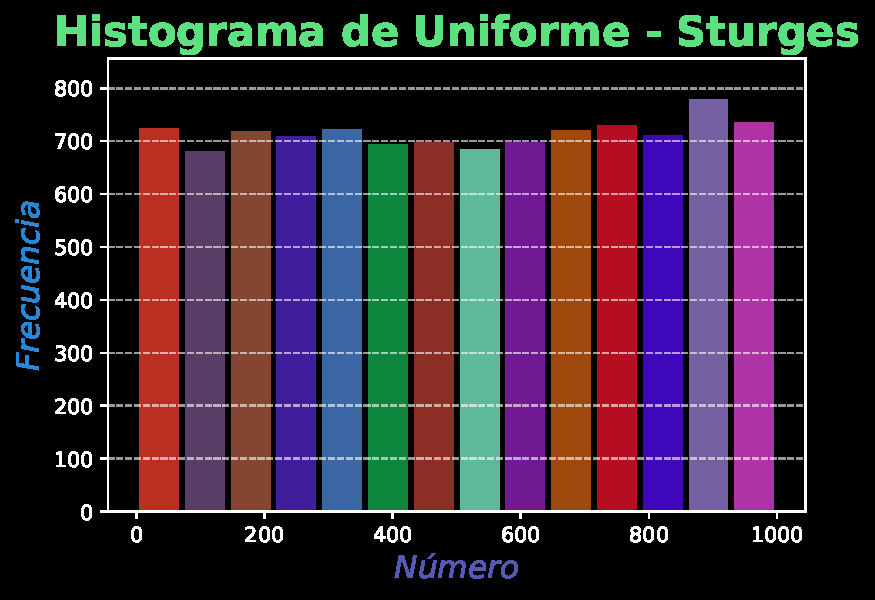
\includegraphics[width=0.7\textwidth]{../transformaciones/hist_uniform_Sturges.pdf}
		\caption{Histograma de números con distribución uniforme.}
		\label{fig:randomsUniforme}
	\end{figure}
	
	
	\section{Transformación de distribución}
	
	En segundo lugar, transformamos los números generados con una distribución uniforme mediante una técnica específica. Esta transformación nos permite obtener un nuevo conjunto de números aleatorios, pero esta vez siguiendo distribuciones de probabilidad distintas, concretamente la distribución normal y la gamma.
	
	\subsection{Transformación a Distribución Normal}
	
	La transformación de variables aleatorias con distribución uniforme a una distribución normal se realiza mediante el uso de la función de error inversa (\textit{inverse error function}), la cual juega un papel crucial en estadística para la transformación de variables aleatorias.
	
	Dado un valor $q$ de una distribución uniforme, el objetivo es encontrar el correspondiente valor en una distribución normal con media $\mu$ y desviación estándar $\sigma$. La transformación se lleva a cabo en dos pasos principales:
	
	\newpage
	La función de error inversa se calcula utilizando una aproximación basada en una fórmula específica. Para un valor $x$, la función se define como:
	
	\[
	\text{inverse\_erf}(x) = \text{sign}(x) \cdot \sqrt{\sqrt{\left(\frac{2}{\pi a} + \frac{\log(1 - x^2)}{2}\right)^2 - \frac{\log(1 - x^2)}{a}} - \left(\frac{2}{\pi a} + \frac{\log(1 - x^2)}{2}\right)}
	\]
	
	donde $a$ es un coeficiente que en esta aproximación toma el valor de 0.147. Esta función permite mapear los valores de $x$ de la distribución uniforme a valores que siguen la función de error, la cual está estrechamente relacionada con la distribución normal.
	
	Con la función de error inversa calculada, el siguiente paso es utilizarla para transformar el cuantil $q$ de la distribución uniforme a un valor que siga una distribución normal estándar, y luego ajustarlo a cualquier media $\mu$ y desviación estándar $\sigma$ deseada. Esto se logra mediante la expresión:
	
	\[
	\text{norm\_ppf}(q, \mu, \sigma) = \mu + \sigma \cdot \sqrt{2} \cdot \text{inverse\_erf}(2q - 1)
	\]
	
	Este método asegura que los valores generados a partir de una distribución uniforme puedan ser transformados efectivamente a valores que siguen una distribución normal con los parámetros especificados.
	
	Dicha transformación se aplicó a los 100,000 números distribuidos uniformemente, se guardó el resultado en un archivo \texttt{randomsNormal.txt}  teniendo a la salida números normalmente distribuidos, como se muestra en el histograma:
	
	\begin{figure}[h]
	 	\centering
	 	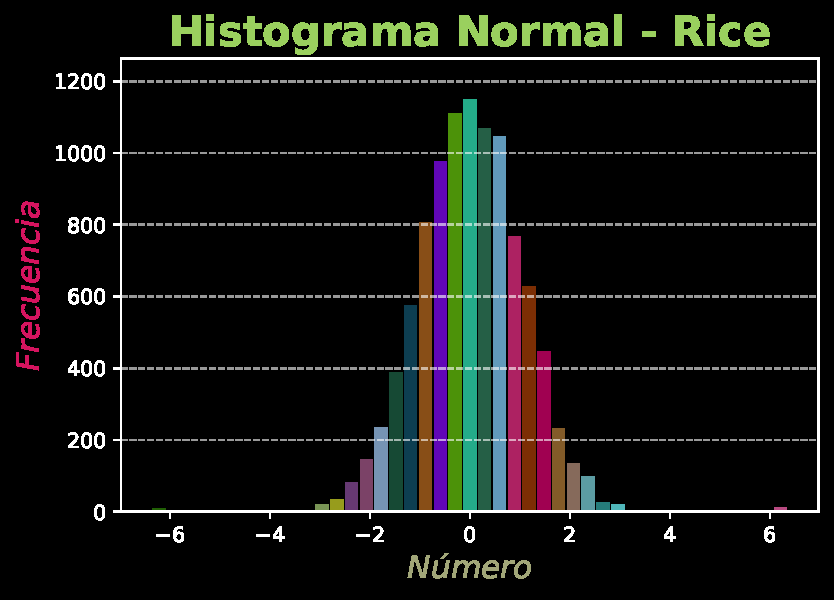
\includegraphics[width=0.70\textwidth]{../transformaciones/hist_normal_Rice.pdf}
	 	\caption{Histograma de números con distribución normal.}
	 	\label{fig:randomsNormal}
	 \end{figure}
	 
	
	\subsection{Transformación a Distribución Gamma}
	 
	 Para generar variables aleatorias que sigan una distribución Gamma con parámetros de forma $a > 1$ y escala $\theta$, utilizamos el siguiente algoritmo:
	 
	 Definimos $\lambda = a - 1$ y calculamos un valor $c$ usando la expresión:
	 \[
	 c = \frac{(a - 1)^{a - 1} e^{1-a}}{\Gamma(a)},
	 \]
	 donde $\Gamma(a)$ es la función Gamma para el parámetro $a$.
	 
	 Repetimos los siguientes pasos hasta que se acepte un candidato:
	 \begin{enumerate}
	 	\item Generamos una variable aleatoria $y$ de una distribución exponencial con parámetro $\lambda$, utilizando la transformación $y = -\frac{\log(1-U)}{\lambda}$, donde $U$ es un número aleatorio uniforme entre 0 y 1.
	 	\item Generamos un número aleatorio uniforme $u$.
	 	\item Aceptamos $y$ si $u \leq \frac{y^{a-1} e^{-y}}{c \lambda^{-a} e^{-\lambda y}}$. En caso contrario, rechazamos $y$ y repetimos el proceso.
	 \end{enumerate}
	 
	 Una vez aceptado, el valor de salida es $y \cdot \theta$, asegurando que la variable aleatoria generada siga una distribución Gamma con los parámetros de forma $a$ y escala $\theta$.
	 
	 De esta manera, obtenemos números con distribución gamma que se almacenaron en \texttt{randomsGamma.txt}. Su transformación la observamos en el siguiente histograma:
	 
	 \begin{figure}[h]
	 	\centering
	 	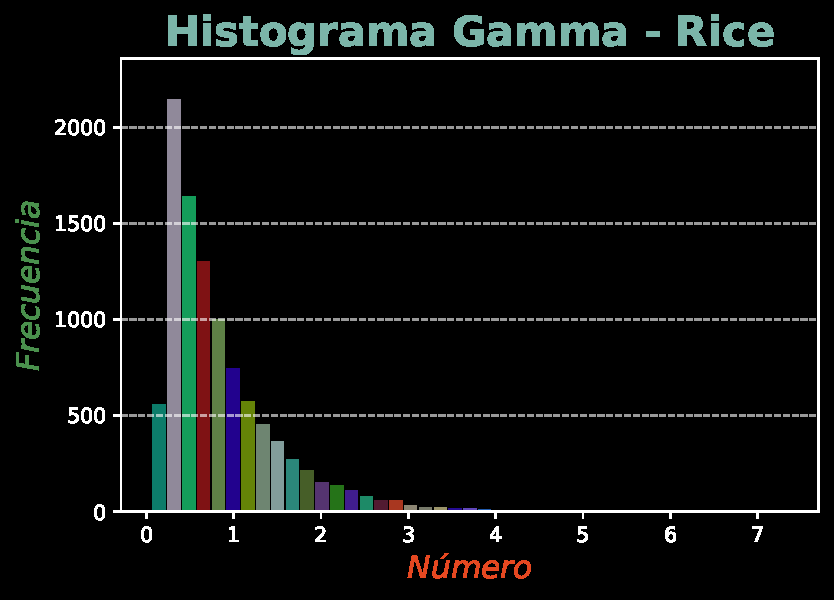
\includegraphics[width=0.70\textwidth]{../transformaciones/hist_gamma_Rice.pdf}
	 	\caption{Histograma de números con distribución gamma.}
	 	\label{fig:randomsGamma}
	 \end{figure}
	 \newpage
	 
	 \section{Métricas de las Distribuciones de Probabilidad}
	 Se realizó una investigación respecto a las expresiones matemáticas que definen a las distribuciones de probabilidad \textit{uniforme, gamma y normal} (las cuales se detallan en el documento \href{https://drive.google.com/file/d/1NWN1bE0bM\_MSOIqLIhVPP\_wj7d1f1rp6/view?usp=drive\_link}{\textbf{Métricas de Probabilidad}}), que se codificaron como sigue para poder aplicarlas en nuestros set de datos anteriores:
	 
	 \subsection{Métricas para un set de datos genérico}
	 \begin{lstlisting}
	 	class DistribucionProbabilidad:
	 	def __init__(self, datos):
		 	self.datos = np.array(datos)
		 	self.n = len(datos)
	 	
	 	def media(self):
	 		return np.mean(self.datos)
	 	
	 	def mediana(self):
	 		return np.median(self.datos)
	 	
	 	def moda(self):
		 	frecuencias = {}
		 	for dato in self.datos:
			 	if dato in frecuencias:
			 		frecuencias[dato] += 1
			 	else:
			 		frecuencias[dato] = 1
		 	
		 	modas = [valor for valor, frecuencia in frecuencias.items() if frecuencia == max(frecuencias.values())]
		 	
		 	if len(modas) == 1:
		 		return modas[0]
		 	else:
		 		return modas
	 	
	 	def media_geometrica(self):
	 		return gmean(self.datos)
	 	
	 	def asimetria(self):
		 	media = self.media()
		 	desv_std = self.desviacion_estandar()
		 	suma_tercero_momento = np.sum((self.datos - media) ** 3)
		 	skewness = (self.n / ((self.n - 1) * (self.n - 2))) * (suma_tercero_momento / (desv_std ** 3))
		 	return skewness
	 	
	 	def rango(self):
	 		return self.datos.max() - self.datos.min()
	 	
	 	def desviacion_estandar(self):
	 		return np.std(self.datos, ddof=1)
	 	
	 	def varianza(self):
	 		return np.var(self.datos, ddof=1)
	 	
	 	def coeficiente_variacion(self):
	 		return self.desviacion_estandar() / self.media()
	 	
	 	def percentil(self, p):
		 	if 0 <= p <= 100:
		 		return np.percentile(self.datos, p)
		 	else:
		 		raise ValueError("El percentil debe estar entre 0 y 100.")
	 	
	 	def cuartil(self, q):
		 	if q in [1, 2, 3]:
		 		return self.percentil(q * 25)
		 	else:
		 		np.nan
	 	
	 	def curtosis(self):
		 	media = self.media()
		 	s = self.desviacion_estandar()
		 	suma_cuarto_momento = np.sum((self.datos - media) ** 4)
		 	curtosis = (self.n * (self.n+1) * suma_cuarto_momento) / ((self.n-1) * (self.n-2) * (self.n-3) * s**4) - (3 * (self.n-1)**2) / ((self.n-2) * (self.n-3))
		 	return curtosis
	 	
	 	def entropia(self):
		 	p, counts = np.unique(self.datos, return_counts=True)
		 	p = counts / len(self.datos)
		 	entropia = -np.sum(p * np.log(p))
		 	return entropia
	 	
	 	def calcular_metricas(self, percentil, cuartil):
		 	resultados = {
		 		'Media': self.media(),
		 		'Mediana': self.mediana(),
		 		'Moda': self.moda(),
		 		'Media Geometrica': self.media_geometrica(),
		 		'Rango': self.rango(),
		 		'Desviacion Estandar': self.desviacion_estandar(),
		 		'Varianza': self.varianza(),
		 		f'Percentil {percentil}': self.percentil(percentil),
		 		f'Cuartil {cuartil}': self.cuartil(cuartil),
		 		'Asimetria': self.asimetria(),
		 		'Coeficiente de Variacion': self.coeficiente_variacion(),
		 		'Curtosis': self.curtosis(),
		 		'Entropia': self.entropia()
		 	}
		 	
		 	for metrica, valor in resultados.items():
			 	print(f"{metrica}: {valor}")
	 \end{lstlisting}
	
	\subsection{Métricas para una Distribución Uniforme}
	\begin{lstlisting}
		class DistribucionUniforme(DistribucionProbabilidad):
		
			def __init__(self, datos):
				super().__init__(datos)
				self.a = min(datos)
				self.b = max(datos)
			
			def media(self):
				return (self.a + self.b)/2
			
			def mediana(self):
				return (self.a + self.b)/2
			
			def media_geometrica(self):
				return super().media_geometrica()
			
			def moda(self):
				return super().moda()
			
			def rango(self):
				return self.b - self.a
			
			def varianza(self):
				return ((self.b - self.a)**2)/12
			
			def desviacion_estandar(self):
				return (((self.b - self.a)**2)/12) ** (1/2)
			
			def coeficiente_variacion(self):
				return ((((self.b - self.a)**2)/12) ** (1/2)) / ((self.a + self.b) / 2)
			
			def percentil(self, num_perc):
				p = num_perc/100
				return self.a + p*(self.b - self.a)
			
			def cuartil(self, num_cuartil):
				num_perc = num_cuartil * 25
				return self.percentil(num_perc)
			
			def asimetria(self):
				return super().asimetria()
			
			def curtosis(self):
				return super().curtosis()
			
			def entropia(self):
				return math.log(self.b - self.a)
			
			def calcular_metricas(self, percentil, cuartil):
				return super().calcular_metricas(percentil, cuartil)
		
	\end{lstlisting}
	
	\subsection{Métricas para una Distribución Normal}
	\begin{lstlisting}
		class DistribucionNormal(DistribucionProbabilidad):
		
			def __init__(self, datos):
				super().__init__(datos)
				self.mu = self.media()
				self.sigma = self.desviacion_estandar()
			
			def media(self):
				return super().media()
			
			def mediana(self):
				return self.mu
			
			def media_geometrica(self):
				return "No aplica"
			
			def moda(self):
				return self.mu
			
			def rango(self):
				return super().rango()
			
			def percentil(self, num_perc):
				p = num_perc/100
				if 0 <= p <= 1:
					valor_z = norm.ppf(p)
					return self.mu + valor_z * self.sigma
				else:
					return np.nan
			
			def cuartil(self, num_cuartil):
				if num_cuartil in [1,2,3,4]:
					c = num_cuartil * 25
					return self.percentil(c)
				
				else:
					return np.nan
			
			def varianza(self):
				return self.sigma**2
			
			def desviacion_estandar(self):
				return super().desviacion_estandar()
			
			def coeficiente_variacion(self):
				if self.mu != 0:
					return self.sigma/self.mu
				else:
					return np.nan
			
			def asimetria(self):
				return super().asimetria()
			
			def curtosis(self):
			return super().curtosis()
			
			def entropia(self):
				return 0.5 * np.log(2 * np.pi * np.e * self.sigma ** 2)
			
			def calcular_metricas(self, percentil, cuartil):
				return super().calcular_metricas(percentil, cuartil)
	\end{lstlisting}
	
	\subsection{Métricas para una Distribución Gamma}
	\begin{lstlisting}
		class DistribucionGamma(DistribucionProbabilidad):
		
			def __init__(self, datos):
				super().__init__(datos)
				self.k, self.theta = self.estimar_params(self.datos)
			
			@staticmethod
			def estimar_params(data):
				def neg_log_likelihood(params, data):
					return -np.sum(gamma.logpdf(data, a=params[0], scale=params[1]))
				
				pesos_iniciales = [1.0, 1.0]
				result = minimize(neg_log_likelihood, pesos_iniciales, args=(data), method='L-BFGS-B', bounds=((0, None), (0, None)))
				
				k_est, theta_est = result.x
				return k_est, theta_est
			
			
			def media(self):
				return self.k * self.theta
			
			def mediana(self):
				return super().mediana()
			
			def media_geometrica(self):
				return super().media_geometrica()
			
			def moda(self):
				if self.k > 1:
					return (self.k - 1) * self.theta
				else:
					return np.nan
			
			def rango(self):
				return super().rango()
			
			def varianza(self):
				return self.k * self.theta**2
			
			def desviacion_estandar(self):
				return (self.k)**(1/2)*self.theta
			
			def coeficiente_variacion(self):
				return 1/(self.k)**(1/2)
			
			def percentil(self, num_perc):
				p = num_perc/100
				return gamma.ppf(p, self.k, scale=self.theta)
			
			def cuartil(self, num_cuartil):
				c = num_cuartil * 25
				return self.percentil(c)
			
			def asimetria(self):
				return super().asimetria()
			
			def curtosis(self):
				return 6/self.k
			
			def entropia(self):
				return self.k + np.log(self.theta) + gammaln(self.k) + (1 - self.k) * psi(self.k)
			
			def calcular_metricas(self, percentil, cuartil):
				return super().calcular_metricas(percentil, cuartil)
	\end{lstlisting}
	
	Así, para los sets de datos \texttt{randomsUniforme.txt}, \texttt{randomsNormal.txt} y \texttt{randomsGamma.txt} se obtuvieron los siguientes resultados:
	
	\newpage
	
	\begin{figure}[h]
		\centering
		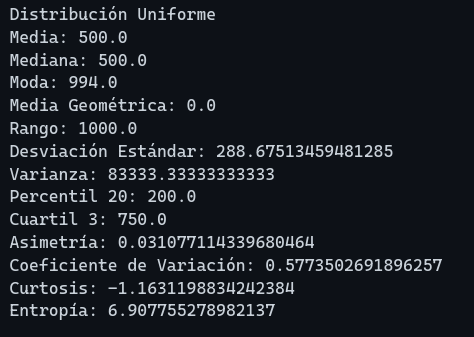
\includegraphics[width=0.49\textwidth]{resultadosUniforme.png}
		\caption{Métricas para el set \texttt{randomsUniforme.txt}.}
		\label{fig:resultados - distribución uniforme}
	\end{figure}
	
	\begin{multicols}{2}
		\begin{minipage}{\linewidth}
			\centering
			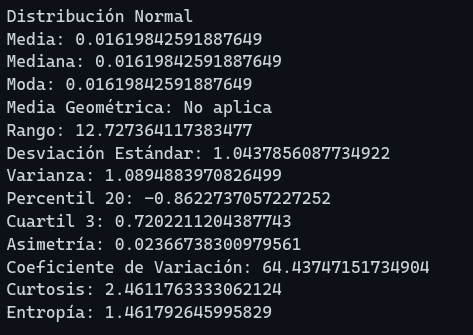
\includegraphics[width=0.9\linewidth]{resultadosNormal.png}
			\captionof{figure}{Métricas para el set \texttt{randomsNormal.txt}.}
			\label{fig:resultados-normal}
		\end{minipage}
		\vfill\columnbreak
		\begin{minipage}{\linewidth}
			\centering
			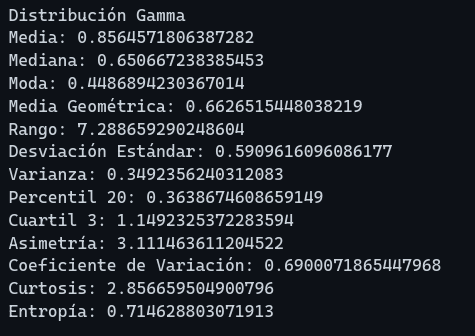
\includegraphics[width=0.9\linewidth]{resultadosGamma.png}
			\captionof{figure}{Métricas para el set \texttt{randomsGamma.txt}.}
			\label{fig:resultados-gamma}
		\end{minipage}
	\end{multicols}
	
	A continuación se analizan los resultados obtenidos al aplicar las métricas a los conjuntos de datos.
	
	\subsection{Análisis de Resultados}
	
	\subsubsection{Para la distribución uniforme}
	Tras aplicar las métricas estadísticas a una muestra de datos generados con una distribución uniforme, hemos obtenido los siguientes resultados:
	
	\begin{itemize}
		\item La \textbf{media} y la \textbf{mediana} tienen el mismo valor de 500.0, lo cual es esperable en una distribución uniforme donde todos los valores tienen la misma probabilidad.
		\item La \textbf{moda} se presenta en 994.0. En una distribución perfectamente uniforme, la moda no está bien definida ya que cada valor es igualmente probable. Sin embargo, debido a variaciones en la muestra, se puede presentar un pico en la frecuencia.
		\item La \textbf{media geométrica} es 0. Este resultado sugiere que la muestra puede contener valores en o cercanos a cero, lo que arrastra el promedio geométrico hacia abajo.
		\item El \textbf{rango} es 1000.0, lo que indica que los datos están esparcidos uniformemente a través de un intervalo amplio.
		\item La \textbf{desviación estándar} y la \textbf{varianza} son coherentes con la fórmula de distribución uniforme $(b-a)^2/12$, reflejando la dispersión de los datos.
		\item El \textbf{coeficiente de variación} es 0.577, lo que puede considerarse bajo, indicando una baja dispersión relativa respecto a la media.
		\item Los valores de \textbf{percentil 20} y \textbf{cuartil 3} son consistentes con lo que se esperaría en una distribución uniforme.
		\item La \textbf{asimetría} se presenta con un valor de 0.031. Esto indica que la distribución de los datos es casi simétrica, con una ligera inclinación hacia la derecha. 
		\item La \textbf{curtosis} negativa sugiere una distribución más achatada que la distribución normal.
		\item La \textbf{entropía} es positiva y está relacionada con el logaritmo del rango de los datos, indicando un grado de incertidumbre asociado a la variabilidad de los datos dentro del rango.
	\end{itemize}
	
	\subsubsection{Para la distribución normal}
	\begin{itemize}
		\item La \textbf{media}, la \textbf{mediana} y la \textbf{moda} tienen valores muy cercanos entre sí, lo que es característico de una distribución normal, que es simétrica alrededor de su media.
		
		\item El \textbf{rango} es aproximadamente 12.73, lo cual nos da una idea de la dispersión total de los datos desde el valor mínimo al máximo.
		
		\item La \textbf{desviación estándar} es de aproximadamente 1.04, indicando que la mayoría de los datos se encuentran dentro de este rango alrededor de la media en una distribución normal.
		
		\item La \textbf{varianza}, siendo el cuadrado de la desviación estándar, refleja la dispersión de los datos y en este caso es aproximadamente 1.09.
		
		\item El \textbf{percentil 20} es aproximadamente -0.86, lo que indica que el 20\% de los valores son menores que este número.
		
		\item El \textbf{cuartil 3} es aproximadamente 0.70, mostrando que el 75\% de los datos están por debajo de este valor.
		
		\item La \textbf{asimetría} tiene un valor cercano a cero (aproximadamente 0.024), lo que confirma la simetría de la distribución. Una distribución perfectamente normal tendría una asimetría de cero.
		
		\item El \textbf{coeficiente de variación} es bastante alto, aproximadamente 64.44, lo que sugiere una variabilidad relativa alta en comparación con la media.
		
		\item La \textbf{curtosis} es aproximadamente 2.46, lo cual es ligeramente superior a 3, que es la curtosis de una distribución normal estándar. Esto indica una distribución un poco más puntiaguda que la normal, con colas más pesadas.
		
		\item La \textbf{entropía}, de aproximadamente 1.46, aunque no es comúnmente discutida en el contexto de la distribución normal, proporciona una medida de incertidumbre o aleatoriedad en la distribución de los datos.
	\end{itemize}
	
	
	\subsubsection{Para la distribución Gamma}
	
	\begin{itemize}
		\item La \textbf{media} es aproximadamente 0.856, lo cual representa el promedio de los valores de la muestra.
		
		\item La \textbf{mediana} de 0.6506 es menor que la media, lo que indica una asimetría hacia la derecha en la distribución.
		
		\item La \textbf{moda} es aproximadamente 0.4486, lo que es esperable en una distribución Gamma asimétrica, donde la moda es menor que la media y la mediana.
		
		\item La \textbf{media geométrica} es aproximadamente 0.6626, siendo relevante en distribuciones sesgadas y generalmente menor que la media aritmética para distribuciones con asimetría positiva.
		
		\item El \textbf{rango}, de aproximadamente 7.29, muestra la diferencia entre los valores máximo y mínimo en la muestra.
		
		\item La \textbf{desviación estándar}, cercana a 0.59, indica la cantidad de variación o dispersión de los valores en la muestra.
		
		\item La \textbf{varianza} es aproximadamente 0.3492, proporcionando otra medida de la dispersión de los datos.
		
		\item El \textbf{percentil 20} es aproximadamente 0.3638, indicando que el 20\% de los valores en la distribución son inferiores a este valor.
		
		\item El \textbf{cuartil 3} es de 1.1492, lo que sugiere que el 75\% de los datos son menores que este valor.
		
		\item La \textbf{asimetría} tiene un valor alto de 3.111, confirmando el sesgo positivo de la distribución y la concentración de la mayoría de los datos hacia el lado izquierdo de la media.
		
		\item El \textbf{coeficiente de variación}, aproximadamente 0.69, muestra una variabilidad relativa en relación con la media de la muestra.
		
		\item La \textbf{curtosis}, de alrededor de 2.856, indica un pico más alto y colas más gruesas en comparación con una distribución normal (curtosis normal = 3).
		
		\item La \textbf{entropía}, de aproximadamente 0.7146, es una medida de la incertidumbre inherente en los resultados de la distribución Gamma.
	\end{itemize}
	
	
	\subsection{Transformaciones al sistema}
	
	Con la intención de seguir caracterizando otros sets de datos y observar como se conservan los sistemas dinámicos cuando a su entrada reciben un conjunto de números aleatorios y se procesan a través de transformaciones \textbf{\textit{lineales y no lineales}} se les aplicó a cada set de datos (\texttt{randomsUniforme.txt, randomsNormal.txt y randomsGamma.txt}) las siguientes funciones:
	
	\newpage
	
	\subsubsection{Transformación lineal: $x^2 - 5x + 7$}
	
	Para la transformación cuadrática con origen en datos uniformemente distribuidos:
	\begin{figure}[h]
		\centering
		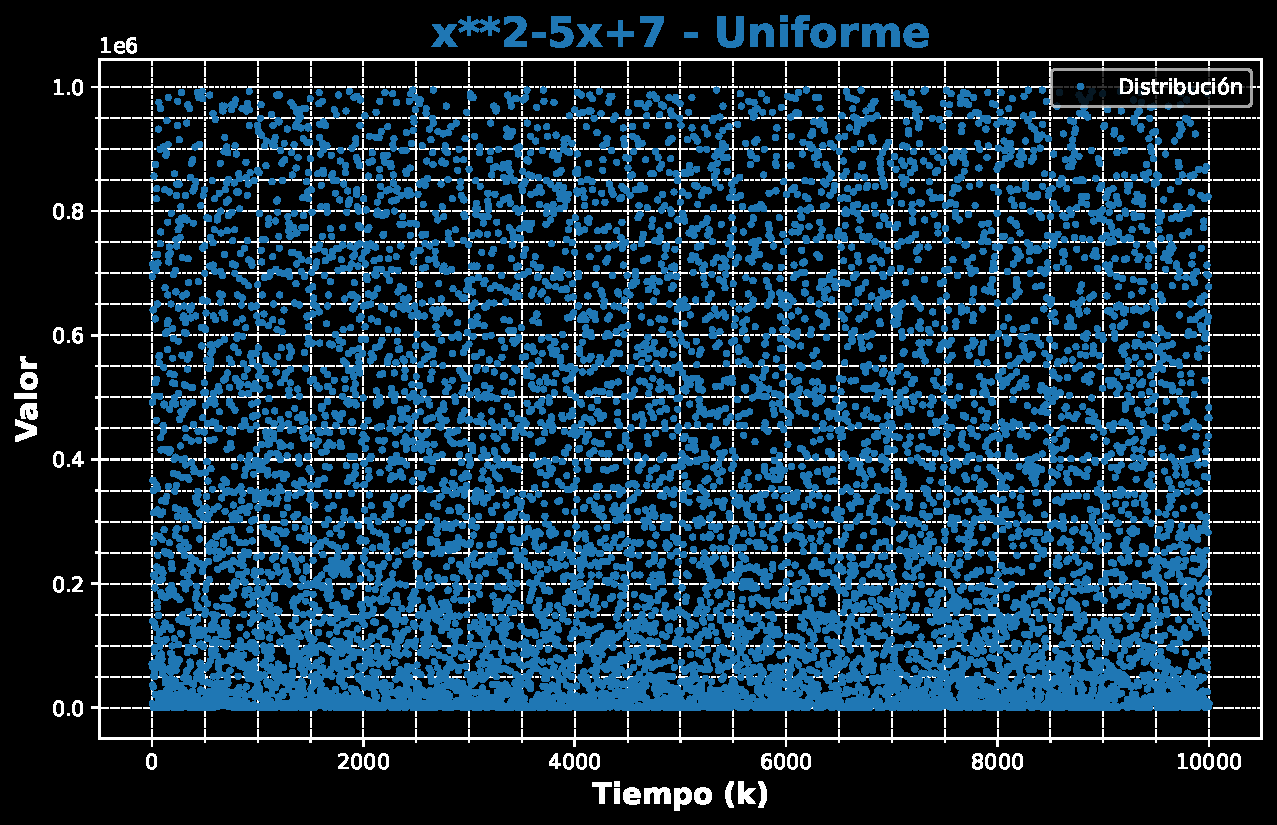
\includegraphics[width=0.7\textwidth]{../transformaciones/cuad_uniforme1.pdf}
		\caption{Gráfica de la serie de tiempo para $x^2 - 5x + 7$ con datos de distribución normal.}
		\label{fig:cuadUnifGraf}
	\end{figure}
	
		\begin{multicols}{2}
			\begin{minipage}{\linewidth}
				\centering
				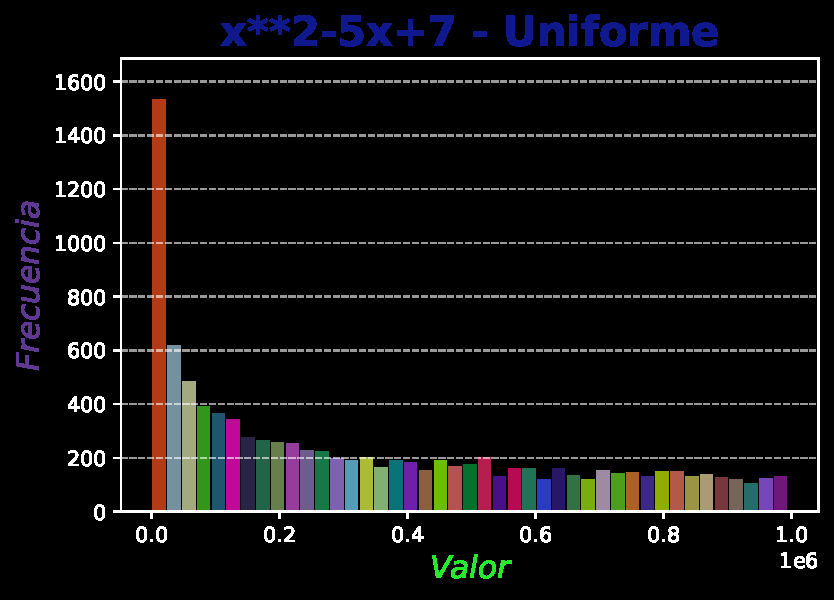
\includegraphics[width=1\linewidth]{../transformaciones/cuad_uniforme2.pdf}
				\captionof{figure}{Histograma.}
				\label{fig:cuadUnifHist}
			\end{minipage}
			\vfill\columnbreak
			\begin{minipage}{\linewidth}
				\centering
				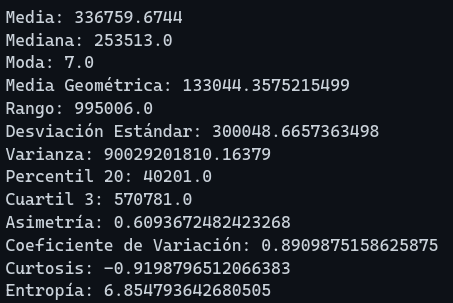
\includegraphics[width=1\linewidth]{../transformaciones/cuad_uniforme3.png}
				\captionof{figure}{Métricas}
				\label{cuadUnifMet}
			\end{minipage}
		\end{multicols}
	
	La serie de tiempo dada presenta una fluctuación que parece uniforme a lo largo de todos sus valores. El histograma asociado y las métricas calculadas revelan las siguientes características:
	
	\begin{itemize}
		\item La \textbf{media} de 336759, siendo el promedio de los datos, sugiere que la suma total de la serie de tiempo es considerablemente alta. En una distribución uniforme ideal, la media y la mediana son cercanas, lo que no se observa en este conjunto de datos.
		
		\item La \textbf{mediana} de 253513, al ser menor que la media, puede indicar que una cantidad significativa de valores de la serie de tiempo son relativamente bajos, lo que podría desplazar la media hacia arriba.
		
		\item La \textbf{moda} de 7 es atípicamente baja y específica en comparación con el rango de los datos. La presencia de una moda tan baja podría ser indicativa de un valor atípico o una acumulación de frecuencias en un punto muy específico de la distribución.
		
		\item La \textbf{media geométrica}, aproximadamente 133041, es relevante en la descripción de los datos cuando la distribución no es simétrica. Su valor inferior a la media aritmética indica una distribución sesgada positivamente.
		
		\item El \textbf{rango} de aproximadamente 995006 muestra que los datos se extienden sobre un intervalo muy amplio.
		
		\item La \textbf{desviación estándar} de 300018 es alta y sugiere que los datos están muy dispersos en relación con la media.
		
		\item El \textbf{percentil 20} de 40201 señala que hay una gran cantidad de datos que son muy bajos en comparación con el valor medio, lo cual apoya la existencia de asimetría positiva.
		
		\item El \textbf{cuartil 3} de 570781 indica que hay una amplia dispersión en los valores superiores de la serie de tiempo. En una distribución uniforme, los cuartiles estarían más equitativamente espaciados.
		
		\item La \textbf{asimetría} positiva de 0.69 sugiere una concentración de datos en el extremo inferior y una cola más larga hacia el lado derecho de la distribución, lo que es indicativo de que hay valores extremadamente altos que están alejando la media de la mediana.
		
		\item El \textbf{coeficiente de variación} de aproximadamente 0.89 indica una alta variabilidad relativa de los datos. Este valor alto sugiere una distribución con mayor dispersión en relación con la media.
		
		\item La \textbf{curtosis} de aproximadamente -0.19 es inferior a la de una distribución normal (con una curtosis de 0), lo que indica que la distribución es más plana que la normal y que tiene colas más ligeras.
		
		\item La \textbf{entropía} de 6.85 es una medida de la incertidumbre y, aunque no proporciona una indicación directa del tipo de distribución, un valor alto sugiere una mayor aleatoriedad en los datos.
	\end{itemize}
	
	Las métricas obtenidas sugieren una distribución con una asimetría positiva y un pico más plano que una distribución normal. La presencia de valores extremos es notable y aleja las características observadas de una distribución uniforme estándar. Con base a estas métricas, los datos parecen alinearse más estrechamente con una distribución que permite valores atípicos y una variabilidad considerable, tal como podría ser una distribución gamma o log-normal, dependiendo de la forma de la distribución observada en los datos.
	
	\newpage
	
	Para la transformación cuadrática con origen en datos normalmente distribuidos:
	\begin{figure}[h]
		\centering
		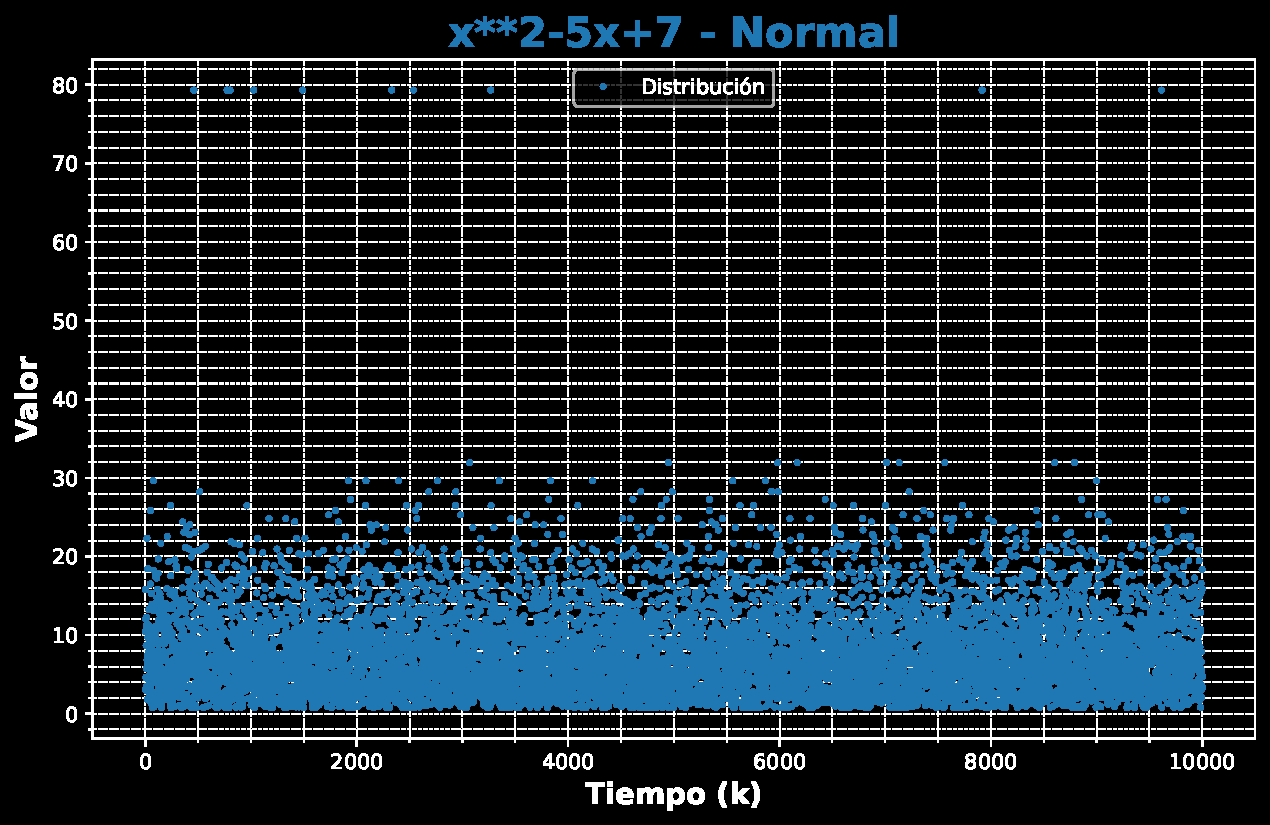
\includegraphics[width=0.7\textwidth]{../transformaciones/cuad_normal1.pdf}
		\caption{Gráfica de la serie de tiempo para $x^2 - 5x + 7$ con datos de distribución uniforme.}
		\label{fig:cuadNormGraf}
	\end{figure}
	
	\begin{multicols}{2}
		\begin{minipage}{\linewidth}
			\centering
			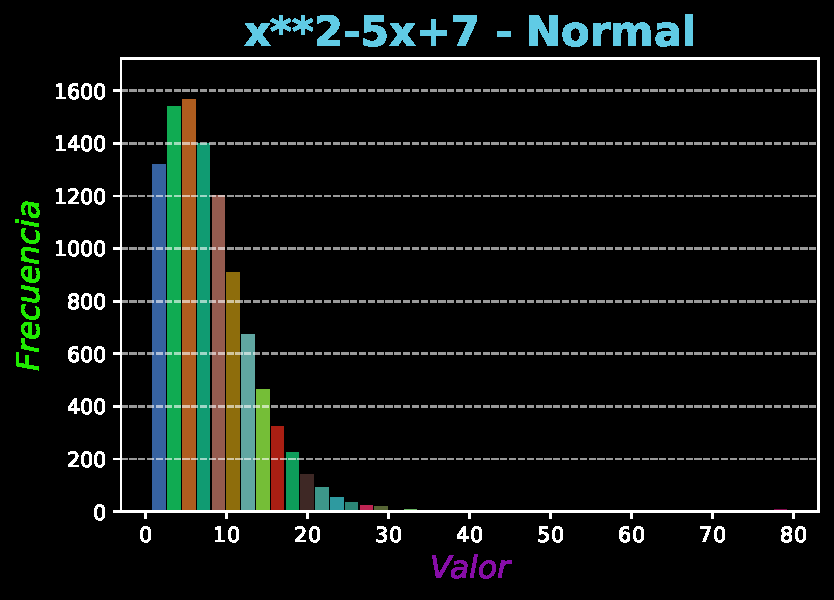
\includegraphics[width=1\linewidth]{../transformaciones/cuad_normal2.pdf}
			\captionof{figure}{Histograma.}
			\label{fig:cuadNormHist}
		\end{minipage}
		\vfill\columnbreak
		\begin{minipage}{\linewidth}
			\centering
			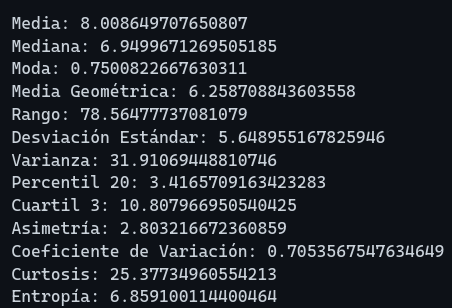
\includegraphics[width=1\linewidth]{../transformaciones/cuad_normal3.png}
			\captionof{figure}{Métricas}
			\label{cuadNormMet}
		\end{minipage}
	\end{multicols}
	
	\begin{itemize}
		\item La \textbf{media} de aproximadamente 8.0 indica el valor promedio de la serie de tiempo. Un valor medio bajo en relación con la amplitud del rango sugiere una concentración de valores bajos.
		
		\item La \textbf{mediana} de 6.9, al estar por debajo de la media, refuerza la indicación de una asimetría positiva, donde más de la mitad de los valores están por debajo del promedio.
		
		\item La \textbf{moda} de 0.75 sugiere que el valor más frecuente es mucho más bajo que la media y la mediana, lo que podría ser indicativo de una acumulación de frecuencias cerca del límite inferior de los datos.
		
		\item La \textbf{media geométrica}, con un valor de aproximadamente 6.25, es menor que la media aritmética, lo que se alinea con una distribución que tiene una asimetría hacia la derecha.
		
		\item El \textbf{rango} es de aproximadamente 78.5, lo que indica la extensión total desde el valor más bajo hasta el más alto en la serie de tiempo.
		
		\item La \textbf{desviación estándar} es de aproximadamente 6.5, lo que muestra una variabilidad considerable alrededor de la media.
		
		\item La \textbf{varianza}, que es el cuadrado de la desviación estándar, nos dice cómo se distribuyen los valores alrededor de la media, y con un valor de aproximadamente 31.9, confirma la dispersión observada.
		
		\item El \textbf{percentil 20} de alrededor de 3.4 indica que el 20\% de los valores son inferiores a este número, lo que nos ayuda a entender la distribución de los valores más bajos.
		
		\item El \textbf{cuartil 3} de aproximadamente 10.8 indica que el 75\% de los datos se encuentran por debajo de este valor, proporcionando una medida de la distribución en el extremo superior.
		
		\item La \textbf{asimetría} con un valor de aproximadamente 2.8 sugiere una fuerte inclinación hacia la derecha, lo que significa que hay una cola más larga de valores hacia el extremo superior de la serie de tiempo.
		
		\item El \textbf{coeficiente de variación} de alrededor de 0.7 indica una variabilidad relativa moderada en relación con el valor medio.
		
		\item La \textbf{curtosis}, de aproximadamente 25.4, es mucho más alta que 0, lo que indica una distribución muy puntiaguda con colas pesadas, o la presencia de valores atípicos significativos.
		
		\item La \textbf{entropía}, con un valor de aproximadamente 6.85, refleja la aleatoriedad en la serie de tiempo. Una entropía alta sugiere una mayor incertidumbre y variabilidad en la distribución de los datos.
	\end{itemize}
	
	La combinación de una alta curtosis y una asimetría significativa sugiere que la distribución de la serie de tiempo no sigue un patrón uniforme ni normal. La presencia de una moda baja y una asimetría positiva sugiere una concentración de valores más bajos y la posibilidad de valores atípicos extremos. Estas características pueden estar asociadas con distribuciones que presentan asimetría positiva y colas pesadas, como ciertas variantes de la distribución gamma o distribuciones log-normales, pero siempre dependiendo de la naturaleza específica de los datos en estudio.
	
	\newpage
	
	Para la transformación cuadrática con origen en datos de distribución gamma:
	\begin{figure}[h]
		\centering
		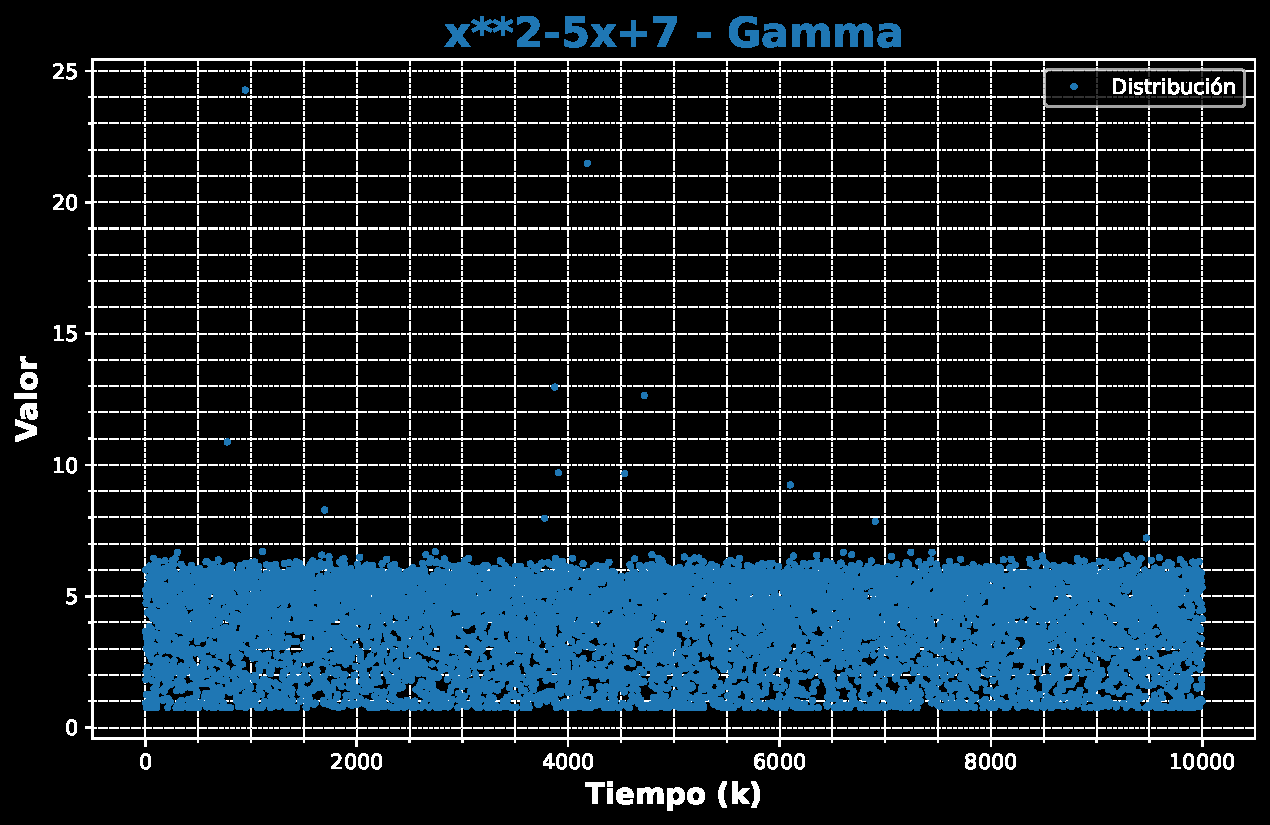
\includegraphics[width=0.7\textwidth]{../transformaciones/cuad_gamma1.pdf}
		\caption{Gráfica de la serie de tiempo para $x^2 - 5x + 7$ con datos de distribución gamma.}
		\label{fig:cuadGammaGraf}
	\end{figure}
	
	\begin{multicols}{2}
		\begin{minipage}{\linewidth}
			\centering
			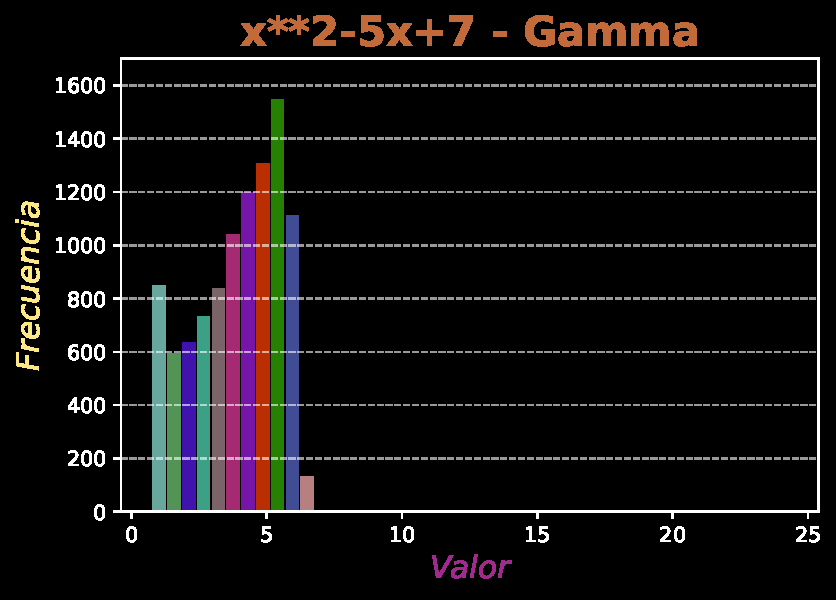
\includegraphics[width=1\linewidth]{../transformaciones/cuad_gamma2.pdf}
			\captionof{figure}{Histograma.}
			\label{fig:cuadGammaHist}
		\end{minipage}
		\vfill\columnbreak
		\begin{minipage}{\linewidth}
			\centering
			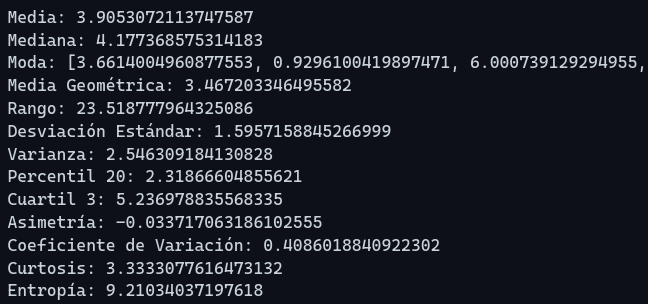
\includegraphics[width=1\linewidth]{../transformaciones/cuad_gamma3.png}
			\captionof{figure}{Métricas}
			\label{cuadGammaMet}
		\end{minipage}
	\end{multicols}
	
	\begin{itemize}
		\item La \textbf{media} de aproximadamente 3.91 indica el promedio de los valores observados en la serie de tiempo, lo que puede sugerir una acumulación de eventos alrededor de este punto.
		
		\item La \textbf{mediana} de 4.12, siendo ligeramente mayor que la media, apunta a una distribución con una cantidad equilibrada de valores por encima y por debajo de este punto central, lo que indica cierta simetría en la distribución de los datos.
		
		\item La \textbf{moda} reporta múltiples valores (3.66, aproximadamente 0.93 y 6.00), indicando que hay varios picos de frecuencia en la distribución de los datos. Esto podría sugerir una distribución multimodal o la presencia de grupos distintos dentro de los datos.
		
		\item La \textbf{media geométrica} de 3.47 es una medida de tendencia central que es típicamente más representativa para datos que no siguen una distribución normal, especialmente cuando la distribución es sesgada.
		
		\item El \textbf{rango} de 23.58 muestra la extensión total de los datos desde el valor más bajo hasta el más alto, lo que indica una variabilidad considerable en la serie de tiempo.
		
		\item La \textbf{desviación estándar} de aproximadamente 1.60 refleja una variabilidad moderada de los datos alrededor de la media, lo que sugiere que los eventos de la serie de tiempo presentan una dispersión consistente.
		
		\item La \textbf{varianza} de aproximadamente 2.55, siendo el cuadrado de la desviación estándar, confirma la dispersión de los datos alrededor de la media.
		
		\item El \textbf{percentil 20} de 2.32 sugiere que el 20\% de los valores son menores a este número, lo que puede ser utilizado para comprender la concentración de los valores más bajos.
		
		\item El \textbf{cuartil 3} de aproximadamente 5.24 indica que el 75\% de los datos son menores que este valor, ofreciendo una visión de la distribución acumulativa hacia el extremo superior.
		
		\item Una \textbf{asimetría} ligeramente negativa de -0.03 sugiere que la serie de tiempo es casi simétrica, con una leve inclinación hacia la izquierda, lo que implica que hay una cantidad ligeramente mayor de eventos por encima de la media.
		
		\item El \textbf{coeficiente de variación} de 0.41 indica que la variabilidad de los datos es proporcionalmente moderada en relación con la media.
		
		\item Una \textbf{curtosis} de aproximadamente 3.33 sugiere una distribución con un pico similar a una distribución normal (curtosis normal = 3), lo que implica que la serie de tiempo no tiene colas inusualmente pesadas ni ligeras.
		
		\item La \textbf{entropía} de 9.21 es una medida de la incertidumbre y aleatoriedad en la serie de tiempo, con un valor más alto sugiriendo una mayor diversidad o aleatoriedad en la distribución de los datos.
	\end{itemize}
	
	En conjunto, estas métricas describen una serie de tiempo con una distribución de valores relativamente simétrica y moderadamente dispersa. La presencia de múltiples modas puede indicar la presencia de subgrupos o comportamientos distintos dentro de la serie de tiempo. La distribución de los datos no parece ser excesivamente sesgada ni puntiaguda, lo que podría ser consistente con una variedad de distribuciones de probabilidad no especificadas sin características extremas o atípicas.
	
	\newpage
	\subsubsection{Transformación no lineal: \( 5\cdot \cos\left(\frac{x}{2}\right) + 7\cdot \cos\left(\frac{x^2}{4}\right) \)}
	
	Para la transformación no lineal con origen en datos de distribución uniforme:
	\begin{figure}[h]
		\centering
		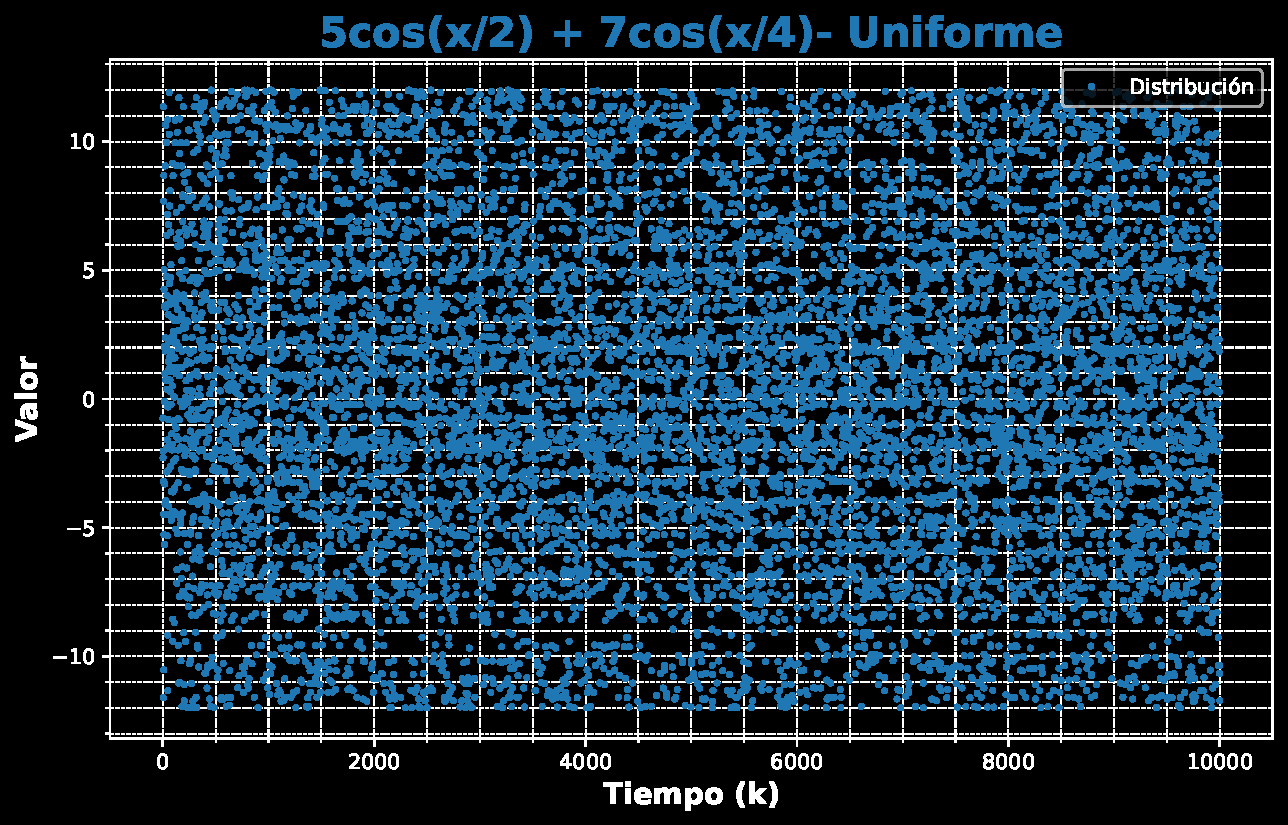
\includegraphics[width=0.7\textwidth]{../transformaciones/per_uniforme1.pdf}
		\caption{Gráfica de la serie de tiempo para \( 5\cdot \cos\left(\frac{x}{2}\right) + 7\cdot \cos\left(\frac{x^2}{4}\right) \) con datos de distribución uniforme.}
		\label{fig:perUnifGraf}
	\end{figure}
	
	\begin{multicols}{2}
		\begin{minipage}{\linewidth}
			\centering
			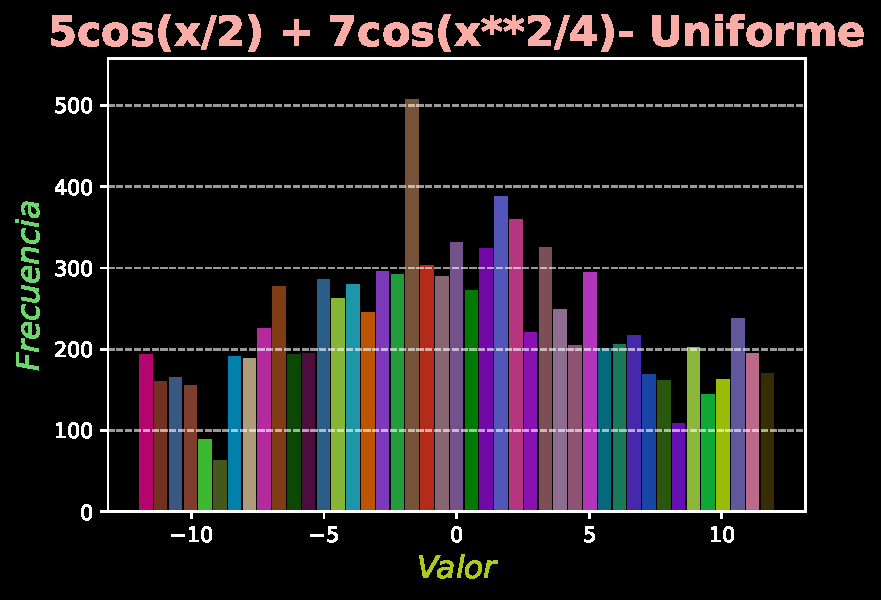
\includegraphics[width=1\linewidth]{../transformaciones/per_uniforme2.pdf}
			\captionof{figure}{Histograma.}
			\label{fig:perUnifHist}
		\end{minipage}
		\vfill\columnbreak
		\begin{minipage}{\linewidth}
			\centering
			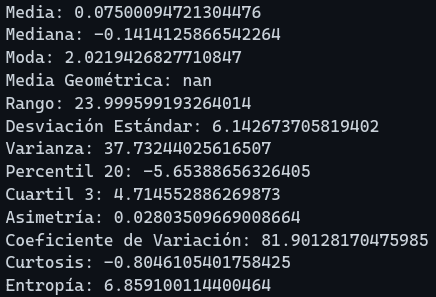
\includegraphics[width=1\linewidth]{../transformaciones/per_uniforme3.png}
			\captionof{figure}{Métricas}
			\label{perUnifMet}
		\end{minipage}
	\end{multicols}
	
	\begin{itemize}
		\item La \textbf{media} cercana a 0.075 sugiere que el promedio de los valores oscila alrededor de cero, lo cual podría indicar una distribución de datos centrada.
		
		\item La \textbf{mediana} de -0.14, siendo ligeramente negativa, muestra que más de la mitad de los valores están por debajo de cero, lo que podría señalar una leve inclinación de los datos hacia valores negativos.
		
		\item La \textbf{moda} de aproximadamente 2.02 indica el valor que ocurre con mayor frecuencia en la serie de tiempo, sugiriendo un pico en la distribución en ese punto.
		
		\item La \textbf{media geométrica} no es aplicable (NaN), típicamente debido a la presencia de valores negativos en los datos que hacen imposible calcular esta métrica.
		
		\item El \textbf{rango} de aproximadamente 23.99 refleja una variabilidad significativa en los datos desde el valor más bajo al más alto.
		
		\item La \textbf{desviación estándar} de alrededor de 6.14 indica que los valores de la serie de tiempo están dispersos de manera considerable respecto a la media.
		
		\item La \textbf{varianza} de aproximadamente 37.73 cuantifica la dispersión observada y es consistente con una desviación estándar elevada.
		
		\item El \textbf{percentil 20} de -5.54 muestra que el 20\% de los valores están concentrados hacia el extremo inferior del rango de la serie de tiempo.
		
		\item El \textbf{cuartil 3} de aproximadamente 4.71 indica que el 75\% de los valores son inferiores a este número, proporcionando una perspectiva de la distribución hacia el extremo superior.
		
		\item Una \textbf{asimetría} de aproximadamente 0.02 sugiere que la serie de tiempo es casi simétrica con una muy ligera inclinación hacia la derecha.
		
		\item El \textbf{coeficiente de variación} de alrededor de 81.90 es extremadamente alto y destaca una variabilidad relativa excepcionalmente grande en relación con la media, lo que puede indicar una amplia gama de comportamientos o estados dentro de la serie de tiempo.
		
		\item Una \textbf{curtosis} de aproximadamente -0.84 es menor que cero, lo que indica una distribución más aplanada que la normal y con colas más ligeras.
		
		\item La \textbf{entropía} de 6.85 muestra la incertidumbre y la aleatoriedad en la distribución de la serie de tiempo, siendo un valor alto que sugiere una gran diversidad en los datos.
	\end{itemize}
	
	Este análisis muestra una serie de tiempo con una distribución de valores que tiene una gran variabilidad y una distribución aplanada. La simetría casi perfecta y la alta variabilidad relativa podrían ser características de una serie de tiempo con influencias aleatorias significativas y sin un patrón o tendencia dominante.
	
	\newpage
	
	Para la transformación no lineal con origen en datos de distribución normal:
	\begin{figure}[h]
		\centering
		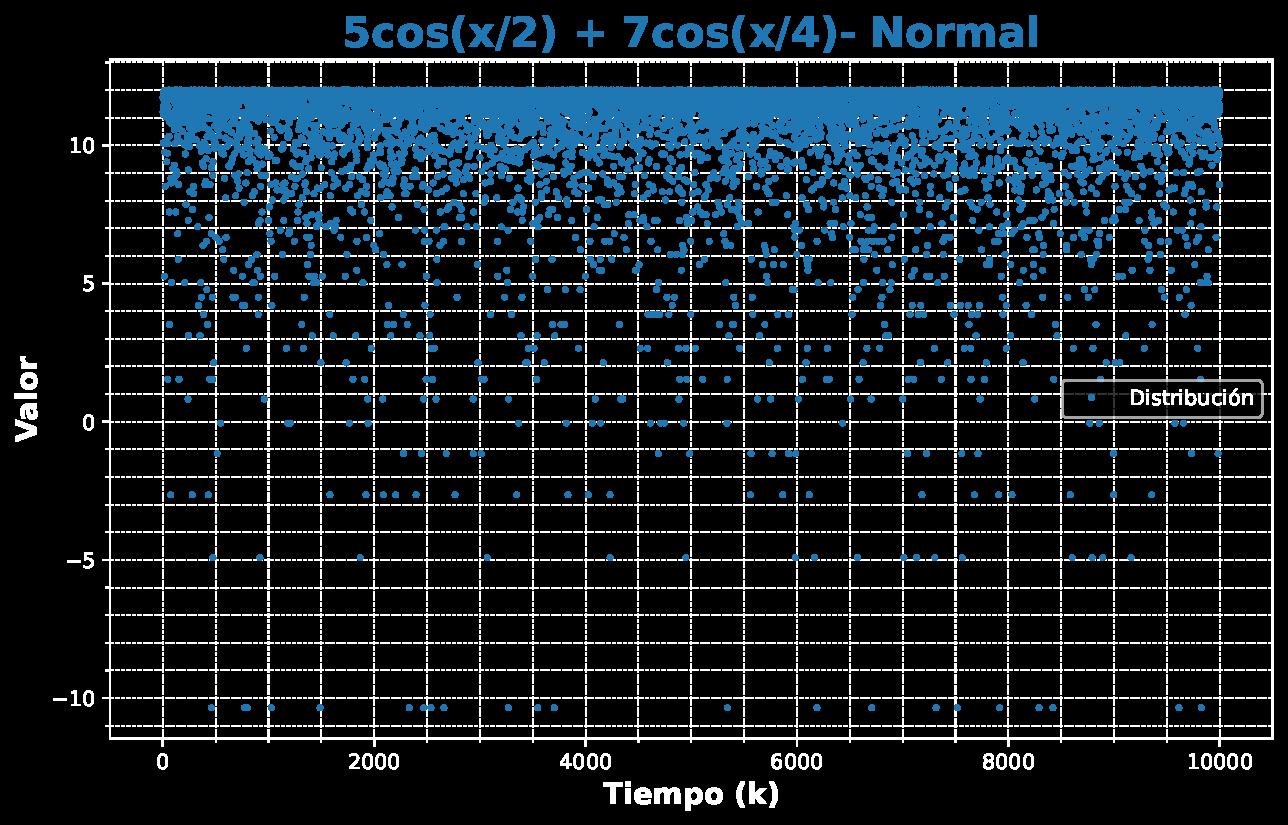
\includegraphics[width=0.7\textwidth]{../transformaciones/per_normal1.pdf}
		\caption{Gráfica de la serie de tiempo para \( 5\cdot \cos\left(\frac{x}{2}\right) + 7\cdot \cos\left(\frac{x^2}{4}\right) \) con datos de distribución normal.}
		\label{fig:perNormGraf}
	\end{figure}
	
	\begin{multicols}{2}
		\begin{minipage}{\linewidth}
			\centering
			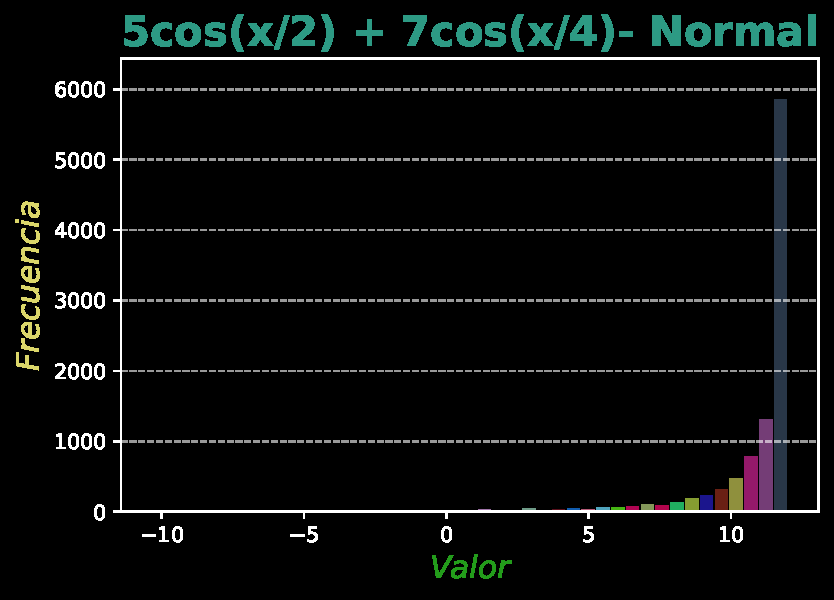
\includegraphics[width=1\linewidth]{../transformaciones/per_normal2.pdf}
			\captionof{figure}{Histograma.}
			\label{fig:perNormHist}
		\end{minipage}
		\vfill\columnbreak
		\begin{minipage}{\linewidth}
			\centering
			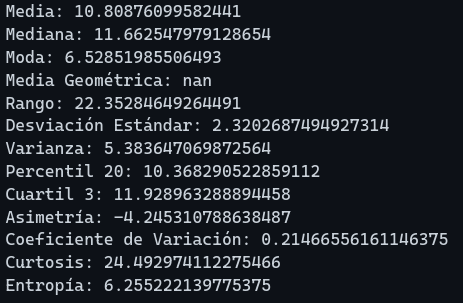
\includegraphics[width=1\linewidth]{../transformaciones/per_normal3.png}
			\captionof{figure}{Métricas}
			\label{perNormMet}
		\end{minipage}
	\end{multicols}
	
	\begin{itemize}
		\item La \textbf{media} de aproximadamente 10.81 indica el valor promedio de la serie de tiempo, lo cual sugiere una tendencia central hacia el extremo superior del rango de los datos.
		
		\item La \textbf{mediana} de 11.66, ligeramente superior a la media, puede señalar una ligera asimetría en los datos, con una concentración de valores más altos.
		
		\item La \textbf{moda} de aproximadamente 5.63 representa el valor más frecuente dentro de la serie de tiempo y parece estar significativamente desplazada de la media y la mediana, lo que indica una distribución de los valores potencialmente bimodal o multimodal.
		
		\item La \textbf{media geométrica} no se puede calcular (NaN) debido a la presencia de valores negativos en los datos.
		
		\item El \textbf{rango} de alrededor de 22.35 muestra una variabilidad significativa entre los valores máximos y mínimos observados en la serie de tiempo.
		
		\item La \textbf{desviación estándar} de aproximadamente 2.32 refleja la cantidad de dispersión que existe alrededor de la media de los datos.
		
		\item La \textbf{varianza} de alrededor de 5.38 cuantifica la dispersión de los datos y, junto con la desviación estándar, confirma la presencia de variabilidad en la serie de tiempo.
		
		\item El \textbf{percentil 20} de 10.36 indica que el 20\% de los datos son menores o iguales a este valor, proporcionando información sobre la distribución acumulativa de los valores inferiores.
		
		\item El \textbf{cuartil 3} de 11.93 refleja el valor por debajo del cual se encuentra el 75\% de los datos, lo que ayuda a entender la concentración de los valores superiores.
		
		\item Una \textbf{asimetría} de -4.24 muestra un sesgo considerable hacia la izquierda, indicando una concentración de valores más hacia el lado derecho de la media.
		
		\item El \textbf{coeficiente de variación} de 0.21 sugiere que la variabilidad de los datos es baja en comparación con la media, lo que indica una relativa uniformidad en la dispersión de los datos.
		
		\item La \textbf{curtosis} extremadamente alta de 24.49 sugiere una distribución muy puntiaguda con colas pesadas, lo que puede implicar la presencia de valores atípicos o un agrupamiento muy denso alrededor de la media.
		
		\item La \textbf{entropía} de 6.25 refleja la incertidumbre y la aleatoriedad de los datos. Un valor más alto indica una mayor diversidad o imprevisibilidad en la distribución de la serie de tiempo.
	\end{itemize}
	
	Estas métricas indican una serie de tiempo con un marcado pico central y una notable simetría hacia la derecha, aunque la asimetría negativa y la curtosis alta sugieren una complejidad subyacente. Estos hallazgos son típicos de series que contienen eventos o comportamientos extremos y valores que se aglomeran en torno a un punto central.
	
	
	\newpage
	
	Para la transformación no lineal con origen en datos de distribución gamma:
	\begin{figure}[h]
		\centering
		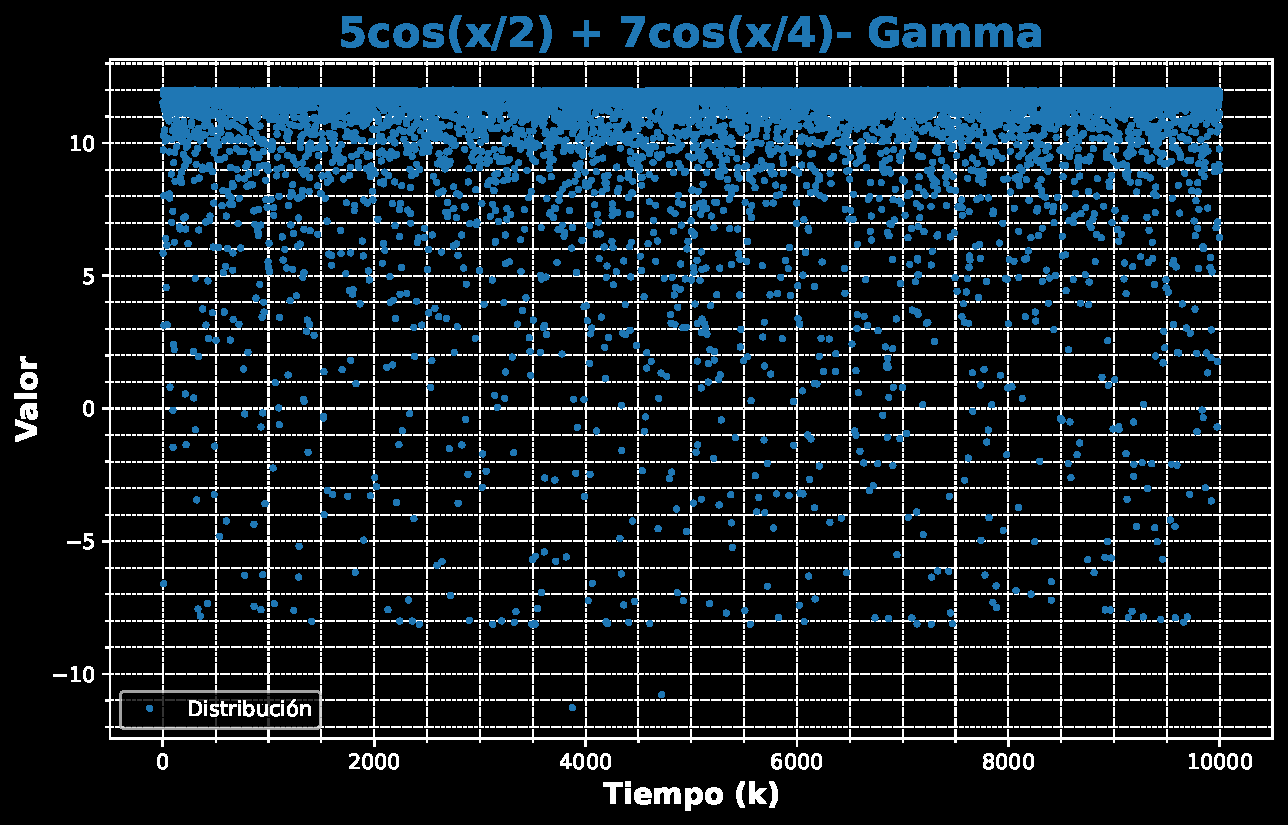
\includegraphics[width=0.7\textwidth]{../transformaciones/per_gamma1.pdf}
		\caption{Gráfica de la serie de tiempo para \( 5\cdot \cos\left(\frac{x}{2}\right) + 7\cdot \cos\left(\frac{x^2}{4}\right) \) con datos de distribución gamma.}
		\label{fig:perGammaGraf}
	\end{figure}
	
	\begin{multicols}{2}
		\begin{minipage}{\linewidth}
			\centering
			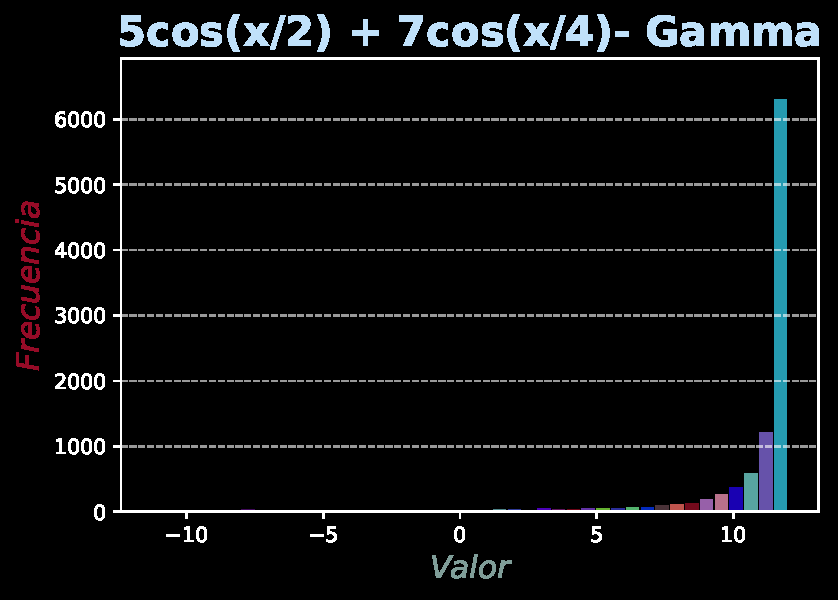
\includegraphics[width=1\linewidth]{../transformaciones/per_gamma2.pdf}
			\captionof{figure}{Histograma.}
			\label{fig:perGammaHist}
		\end{minipage}
		\vfill\columnbreak
		\begin{minipage}{\linewidth}
			\centering
			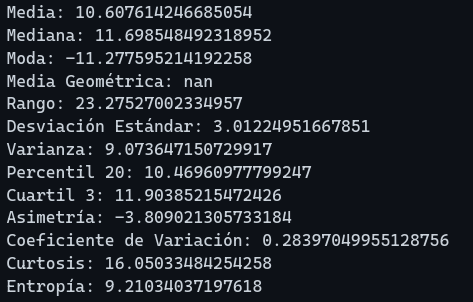
\includegraphics[width=1\linewidth]{../transformaciones/per_gamma3.png}
			\captionof{figure}{Métricas}
			\label{perGammaMet}
		\end{minipage}
	\end{multicols}
	
	\begin{itemize}
		\item La \textbf{media} de aproximadamente 10.61 puede sugerir que la distribución de los valores tiende a ser mayor en comparación con el punto de equilibrio de cero, indicando una posible acumulación de eventos en el lado positivo.
		
		\item La \textbf{mediana} de 11.69, mayor que la media, indica que más de la mitad de los valores están por encima del promedio, reforzando la idea de que hay una tendencia hacia valores mayores en la serie de tiempo.
		
		\item La \textbf{moda} de -11.28 es inusualmente baja y distinta de la media y la mediana, lo cual es característico de una distribución que podría ser bimodal o tener un comportamiento atípico en su distribución de valores.
		
		\item La \textbf{media geométrica} no se calcula (NaN), lo que comúnmente ocurre debido a la presencia de valores negativos en los datos, lo que impide el cálculo de esta métrica.
		
		\item El \textbf{rango} de 23.25 muestra la diferencia entre los valores máximo y mínimo en la serie de tiempo, lo que indica una extensa variabilidad de los datos.
		
		\item La \textbf{desviación estándar} de aproximadamente 3.01 sugiere una dispersión considerable de los datos alrededor de la media, lo que indica una amplia gama de comportamientos o valores en la serie de tiempo.
		
		\item La \textbf{varianza} de aproximadamente 9.07, como el cuadrado de la desviación estándar, cuantifica la dispersión de los datos y es consistente con una desviación estándar alta.
		
		\item El \textbf{percentil 20} de 10.47 muestra que el 20\% de los datos son menores o iguales a este valor, proporcionando una indicación de la distribución acumulativa de los valores inferiores.
		
		\item El \textbf{cuartil 3} de 11.90 indica que el 75\% de los valores están por debajo de este número, lo que ayuda a entender la concentración de los valores superiores en la serie de tiempo.
		
		\item Una \textbf{asimetría} de -3.89 sugiere un sesgo significativo hacia la izquierda, lo que indica una cola larga de eventos hacia el lado izquierdo de la distribución.
		
		\item El \textbf{coeficiente de variación} de 0.28 sugiere una baja variabilidad relativa de los datos en comparación con la media, lo que podría indicar una concentración de valores alrededor de la media.
		
		\item La \textbf{curtosis} extremadamente alta de 16.05 indica una distribución con un pico muy agudo y colas pesadas, lo que puede sugerir la presencia de valores extremos o comportamientos muy concentrados alrededor de la media.
		
		\item La \textbf{entropía} de 2.91 refleja la incertidumbre y la diversidad en la distribución de la serie de tiempo, con un valor más alto indicando una mayor imprevisibilidad o variedad en los datos.
	\end{itemize}
	
	Estos resultados nos llevan a concluir que estamos observando una serie de tiempo con una distribución de datos que tiene una asimetría significativa hacia la izquierda y una curtosis muy elevada. Estas características sugieren una serie con una gran cantidad de valores concentrados alrededor de un punto central y una posible presencia de valores atípicos que influyen en la forma de la distribución.
	
	
	\section{Caminante Aleatorio}
	
	Con base en los datos generados con una distribución uniforme (\texttt{randomsUniforme.txt}), distribución normal (\texttt{randomsNormal.txt}) y distribución gamma \texttt{(randomsGamma.txt)} se plantea crear la animación del caminante aleatorio con el fin de observar su comportamiento al ser alimentado con números aleatorios basados en estas de probabilidad, y analizar las series de tiempo (mediante las métricas) generadas por:
	
	\begin{itemize}
		\item Dirección tomada.
		\item Distancia recorrida en cada paso.
		\item Choques con pared
		\item Posición (x,y) en el plano a lo largo del tiempo.
	\end{itemize}
	
	\subsection{Procedimiento}
	
	Se crea una cuadrícula en la que se posicionan n caminantes aleatorios (cuyo número fue definido por el usuario) en una posición aleatoria.
	
	Luego, se crea una instancia para cada caminante, cargando el archivo de la distribución de probabilidad seleccionada.
	
	En tercer lugar, se elige un número random que representará la dirección en la que se moverá el caminante, como se muestra en la figura \ref{fig:dir-paredes}. Posteriormente se elige otro número random que representará la distancia que el caminante recorrerá en la dirección ya seleccionada.
	
	A su vez, por cada movimiento, se registrán los choques que se dan con la pared, cuyo índice es el que se muestra en la figura \ref{fig:dir-paredes}. Así como su posición x,y en el mapa.
	
		\begin{figure}[h]
			\centering
			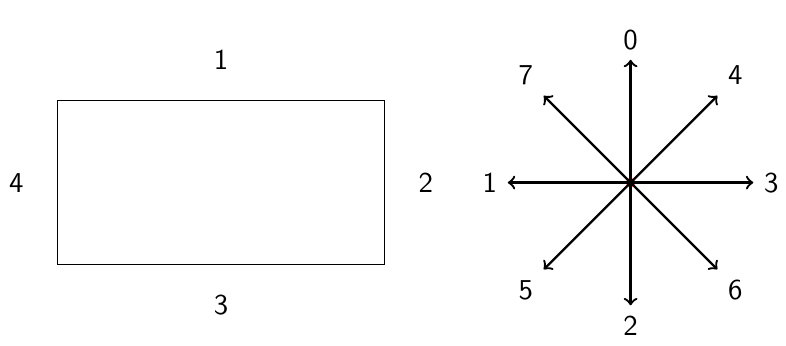
\includegraphics[width=0.6\linewidth]{rectangulo.png}
			\caption{Índices de las paredes y las direcciones.}
			\label{fig:dir-paredes}
		\end{figure}
	
	
	\textit{Nota:} Por simplicidad, aunque se observen más caminantes aleatorios en cada animación, se analizará solamente al de color \textbf{\textit{blanco}}.
	
	 \subsection{Caminante Aleatorio con Distribución Uniforme}
	 
	 \begin{center}
	 	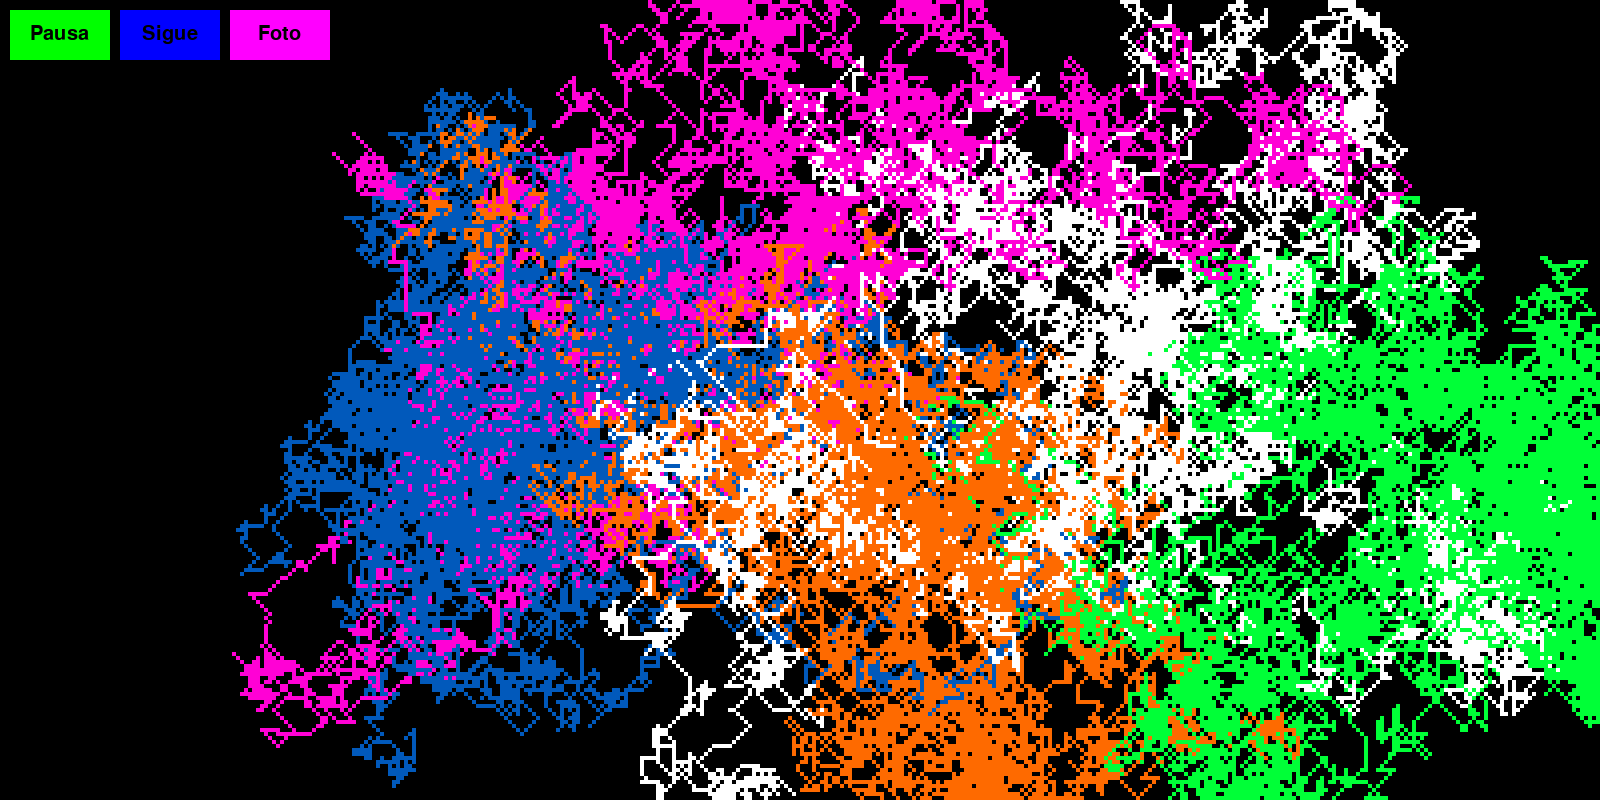
\includegraphics[width=0.8\linewidth]{walkerUniforme.png}
	 	\captionof{figure}{Caminante Aleatorio - Distribución Uniforme}
	 	\label{walkerUniforme}
	 \end{center}
	 
	 \subsubsection{Direcciones}
	 \begin{figure}[h]
	 	\centering
	 	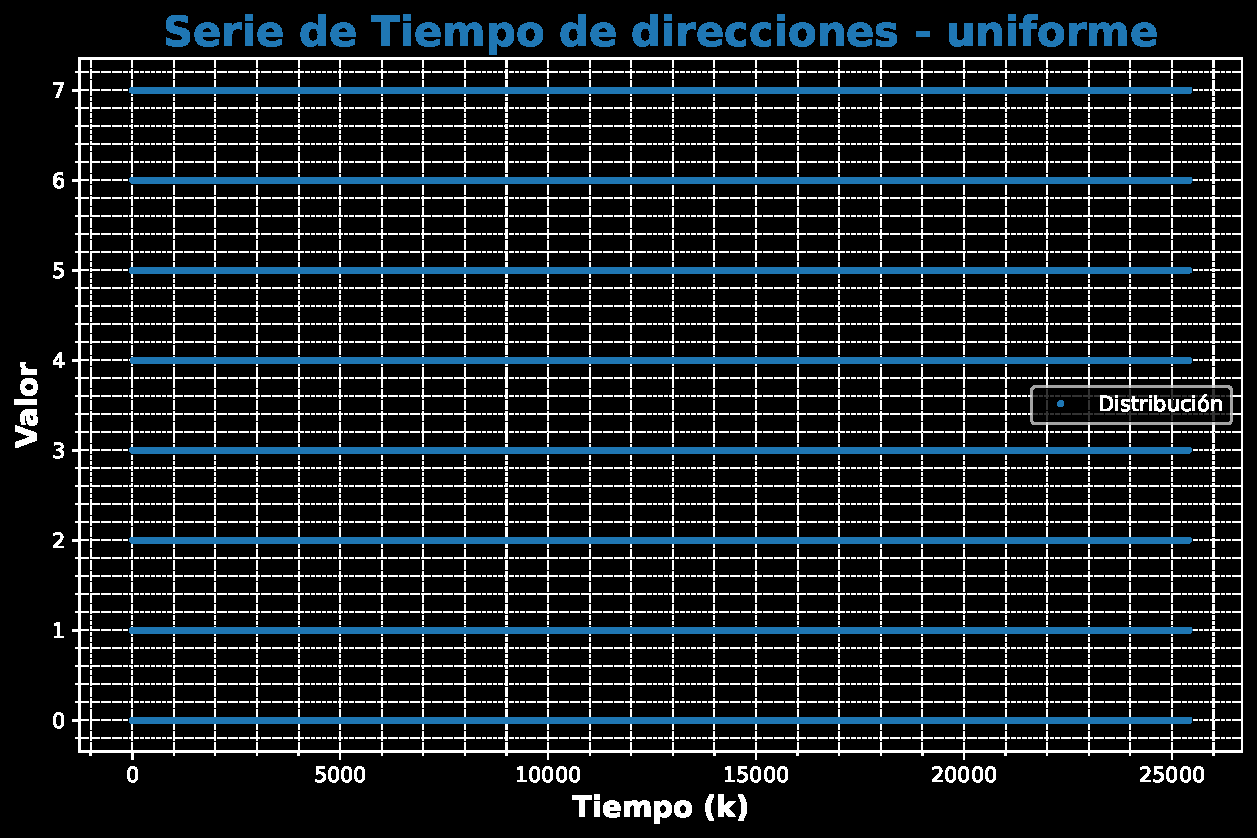
\includegraphics[width=0.7\textwidth]{graf_direcciones_uniforme.pdf}
	 	\caption{Gráfica de la serie de tiempo para las direcciones del caminante con distribución uniforme.}
	 	\label{fig:direcUnifGraf}
	 \end{figure}
	 \begin{multicols}{2}
	 	\begin{minipage}{\linewidth}
	 		\centering
	 		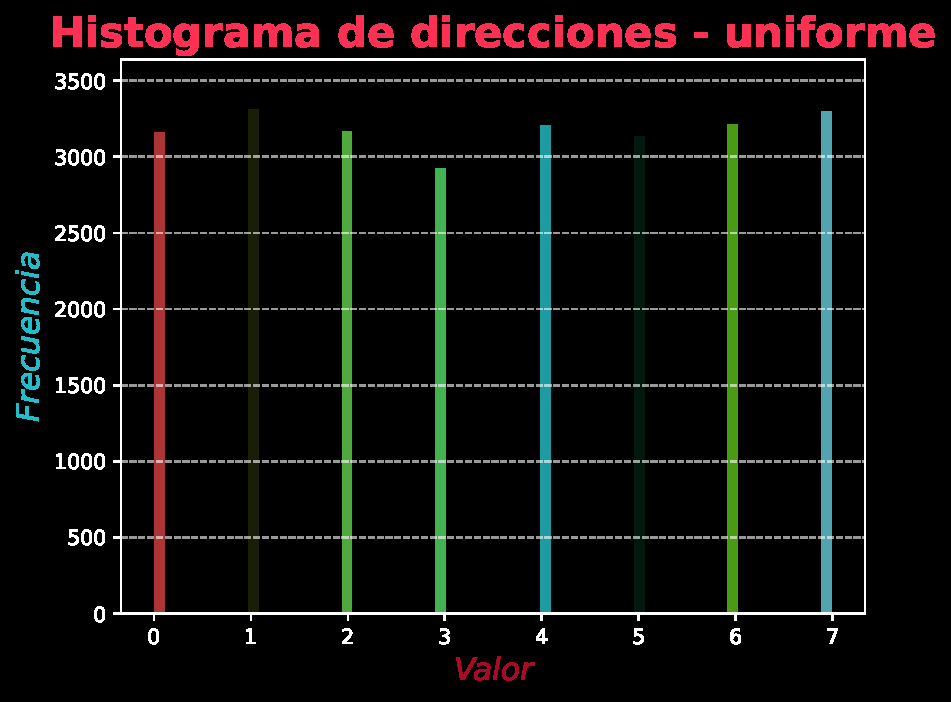
\includegraphics[width=1\linewidth]{hist_direcciones_uniforme.pdf}
	 		\captionof{figure}{Histograma.}
	 		\label{fig:direcUnifHist}
	 	\end{minipage}
	 	\vfill\columnbreak
	 	\begin{minipage}{\linewidth}
	 		\centering
	 		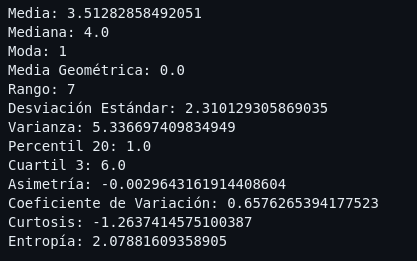
\includegraphics[width=1\linewidth]{u1.png}%
	 		\captionof{figure}{Métricas}
	 		\label{direcUnifMet}
	 	\end{minipage}
	 \end{multicols}
	 
	 \begin{itemize}
	 	
	 	\item La \textbf{mediana} de 4.0, que es el valor central de los datos, sugiere que la mitad de las distancias son mayores que 4.0 y la otra mitad son menores, lo que indica un equilibrio en la distribución de las direcciones.
	 	
	 	\item La \textbf{moda} de 1 sugiere que el valor más comúnmente observado para la distancia en la serie de tiempo es 1, lo que podría indicar una frecuencia alta de este resultado específico o un posible punto de concentración en los datos.
	 	
	 	\item La \textbf{media geométrica} es 0.0, lo cual generalmente significa que hay valores de cero en los datos, afectando este promedio.
	 	
	 	\item El \textbf{rango} de 7 muestra la extensión completa de los datos desde el valor más bajo hasta el más alto registrado.
	 	
	 	\item Una \textbf{asimetría} de aproximadamente -0.0029 sugiere que la distribución es muy simétrica, con una ligera inclinación hacia la izquierda.
	 	
	 	\item El \textbf{coeficiente de variación} de 0.6576 refleja una variabilidad relativa moderada en comparación con la media, lo que podría indicar un grado de homogeneidad en las distancias registradas.
	 	
	 	\item La \textbf{curtosis} de -1.25, es típica de la distribución uniforme.
	 	
	 	\item La \textbf{entropía} de 2.07, similar al de aplicar el $ln(b-a) = ln(7)$, que es la métrica de la entropía en la distribución uniforme.
	 \end{itemize}
	 
	 El análisis de estas métricas sugiere una serie de tiempo de distancias con una distribución bastante simétrica y un grado de variabilidad moderado. El perfil aplanado de la distribución, junto con la simetría y el rango de los datos, puede indicar una distribución \textbf{uniforme} de las distancias.
	  

	\subsubsection{Distancias}
	 \begin{figure}[h]
	 	\centering
	 	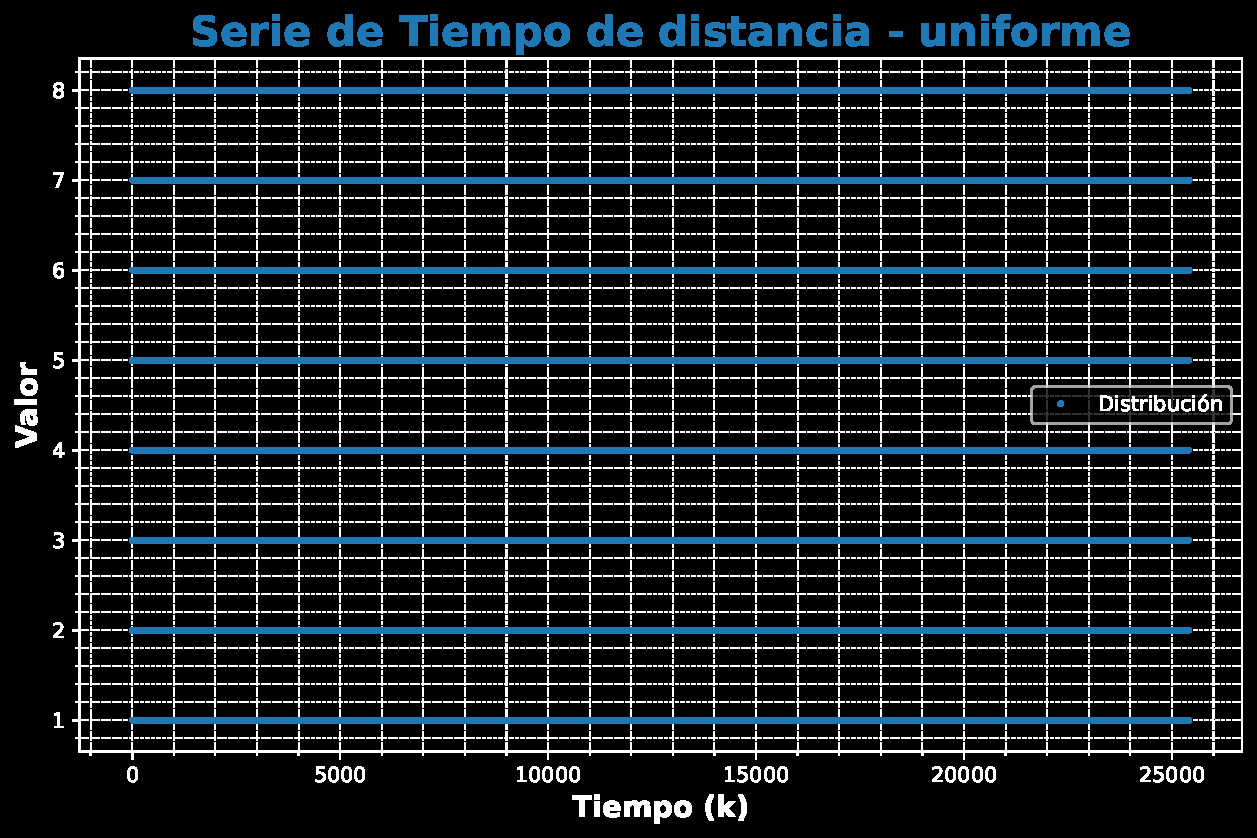
\includegraphics[width=0.6\textwidth]{graf_distancia_uniforme.pdf}
	 	\caption{Gráfica de la serie de tiempo para las distancias del caminante con distribución uniforme.}
	 	\label{fig:distUnifGraf}
	 \end{figure}
	 \begin{multicols}{2}
	 	\begin{minipage}{\linewidth}
	 		\centering
	 		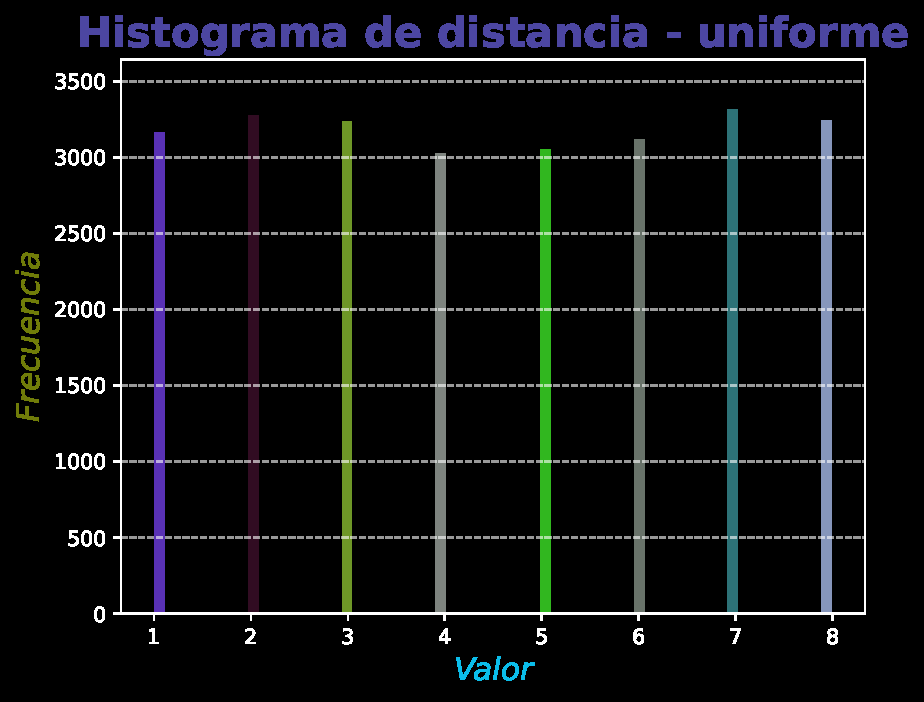
\includegraphics[width=1\linewidth]{hist_distancia_uniforme.pdf}
	 		\captionof{figure}{Histograma.}
	 		\label{fig:distUnifHist}
	 	\end{minipage}
	 	\vfill\columnbreak
	 	\begin{minipage}{\linewidth}
	 		\centering
	 		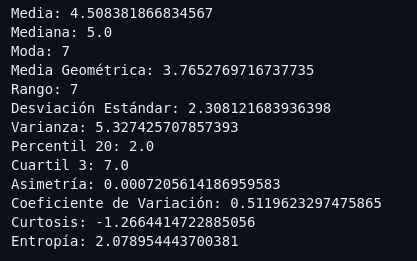
\includegraphics[width=1\linewidth]{u2.png}%
	 		\captionof{figure}{Métricas}
	 		\label{distUnifMet}
	 	\end{minipage}
	 \end{multicols}
	 
	 \begin{itemize}
	 	\item La \textbf{mediana} de 5.0, que coincide con el valor medio del rango, indica una distribución simétrica de los valores en torno a este punto central.
	 	\item El \textbf{rango} de 7 sugiere que los valores de la serie de tiempo se extienden uniformemente a lo largo del espectro de datos posible.
	 	\item La \textbf{desviación estándar} de aproximadamente 2.30, junto con la varianza de 5.32, señalan una dispersión moderada de los valores alrededor de la media.
	 	\item El \textbf{percentil 20} y el \textbf{cuartil 3}, ambos con valores de 2.0 y 7.0 respectivamente, refuerzan la idea de una distribución uniforme, donde los valores están igualmente dispersos a lo largo del intervalo.
	 	\item La \textbf{asimetría} cercana a cero sugiere que la serie de tiempo es casi perfectamente simétrica.
	 	\item El \textbf{coeficiente de variación} de 0.51 indica una variabilidad relativa moderada con respecto a la media de la serie de tiempo.
	 	\item Una \textbf{curtosis} negativa de -1.26 es típica de la distribución uniforme.
	 	\item La \textbf{entropía} de 2.07, que es relativamente baja, sugiere que hay un menor grado de incertidumbre o aleatoriedad en la distribución de los datos y es similar al de aplicar el $ln(b-a) = ln(8-1)= ln(7)$, que es la métrica de la entropía en la distribución uniforme
	 \end{itemize}
	 
	 Las métricas proporcionadas son características de una distribución que se distribuye de manera bastante \textbf{uniforme} a lo largo de su rango, con una varianza moderada y sin sesgo aparente en ninguna dirección.
	 
	 
	 \subsubsection{Posiciones}
	 \begin{figure}[h]
	 	\centering
	 	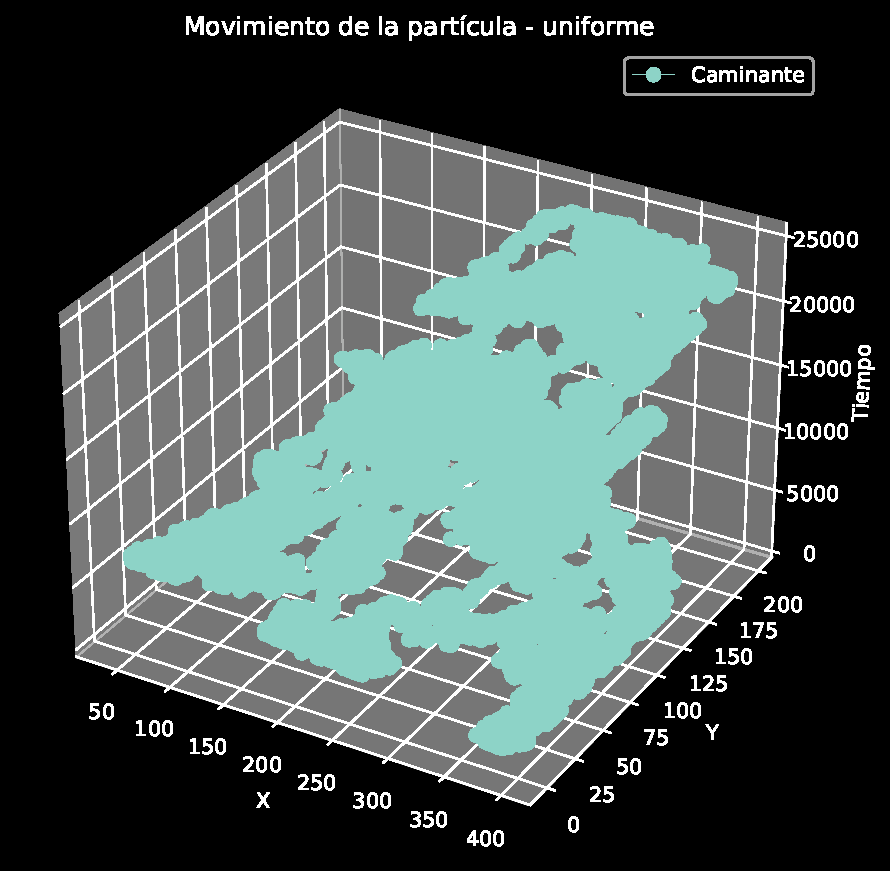
\includegraphics[width=0.5\textwidth]{graf_posiciones_uniforme.pdf}
	 	\caption{Gráfica de la serie de tiempo para las posiciones del caminante con distribución uniforme.}
	 	\label{fig:posUnifGraf}
	 \end{figure}
	 
	 \newpage
	 \begin{multicols}{2}
	 	\begin{minipage}{\linewidth}
	 		\centering
	 		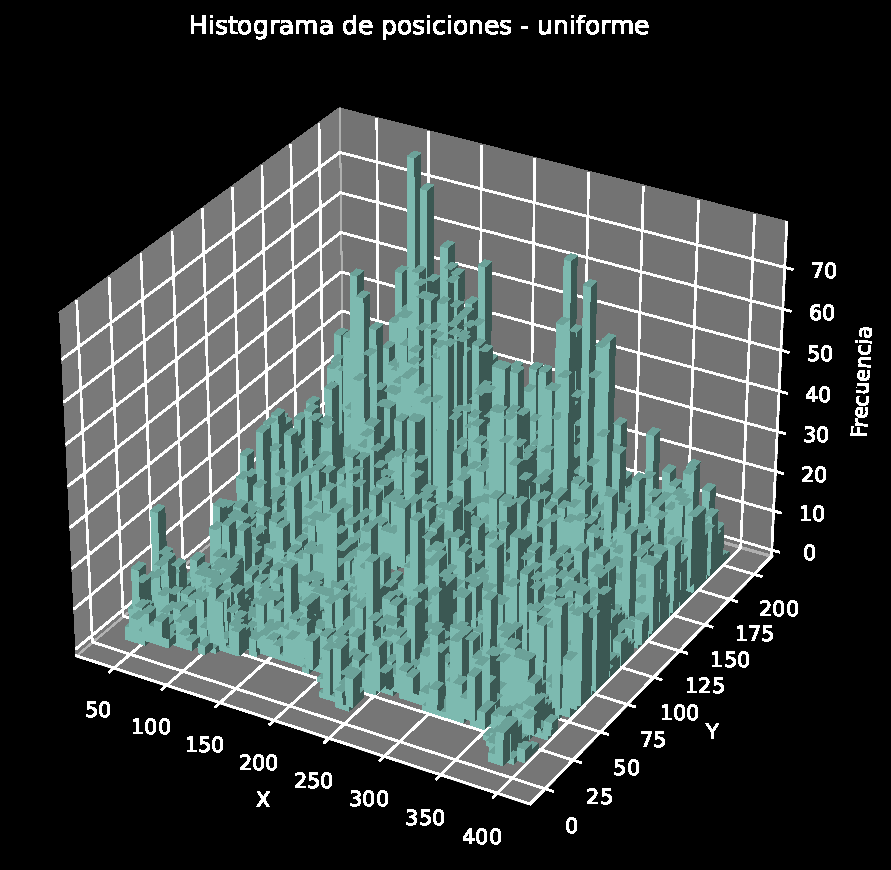
\includegraphics[width=0.8\linewidth]{hist_posiciones_uniforme.pdf}
	 		\captionof{figure}{Histograma.}
	 		\label{fig:posUnifHist}
	 	\end{minipage}
	 	\vfill\columnbreak
	 	\begin{minipage}{\linewidth}
	 		\centering
	 		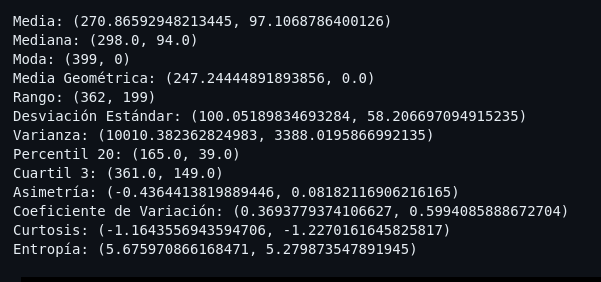
\includegraphics[width=1\linewidth]{u3.png}%
	 		\captionof{figure}{Métricas}
	 		\label{posUnifMet}
	 	\end{minipage}
	 \end{multicols}
	 
	 \begin{itemize}
	 	\item La \textbf{media} en las coordenadas (270.86, 94.12), sugiere que el centro de masa de la distribución de posiciones está situado en esta localización en el espacio bidimensional.
	 	
	 	\item La \textbf{mediana} en las coordenadas (298.0, 94.0), muy cercana a la media, indica que la mitad de las posiciones caen por debajo de este valor y la otra mitad por encima, lo que apunta a una distribución equitativa en ambas direcciones del plano.
	 	
	
	 	\item El \textbf{rango}, con valores máximos en (362, 189), muestra la extensión total de los datos en el espacio bidimensional.
	 	
	 	\item La \textbf{desviación estándar}, con valores aproximados de (106.81, 56.20), refleja la dispersión de las posiciones respecto a la media en cada dirección.
	 	
	 	\item Una \textbf{asimetría} negativa de aproximadamente -4.30 en la dirección 'x' y positiva de 0.08 en la dirección 'y' sugiere una cola más pesada hacia el lado izquierdo en la dirección 'x' y una distribución más simétrica en la dirección 'y'.
	 	
	 	\item El \textbf{coeficiente de variación} de aproximadamente 0.39 en 'x' y 0.59 en 'y', indica una variabilidad relativa menor en la dirección 'x' en comparación con 'y'.
	 	
	 	\item La \textbf{curtosis}, con un valor de 1.65 en 'x' y 28.37 en 'y', sugiere una distribución más plana de lo normal en 'x' y una distribución muy puntiaguda con colas pesadas en 'y'.
	 	
	 	\item La \textbf{entropía} de 6.57 en 'x' y 2.52 en 'y', mide el grado de incertidumbre y aleatoriedad en la distribución de las posiciones en ambas direcciones, siendo relativamente alta en 'x' e indicando más uniformidad en 'y'.
	 \end{itemize}
	 
	 Los valores indican una distribución con una dispersión considerable y una asimetría notable en la dirección 'x', mientras que en la dirección 'y', los valores sugieren una mayor concentración alrededor de la moda con colas pesadas. Estas características podrían alinearse con una serie de tiempo que contiene un área de actividad concentrada y comportamientos atípicos en determinadas regiones del espacio bidimensional analizado.
	 
	 
	 \newpage
	 \subsubsection{Choques contra paredes}
	 \begin{figure}[h]
	 	\centering
	 	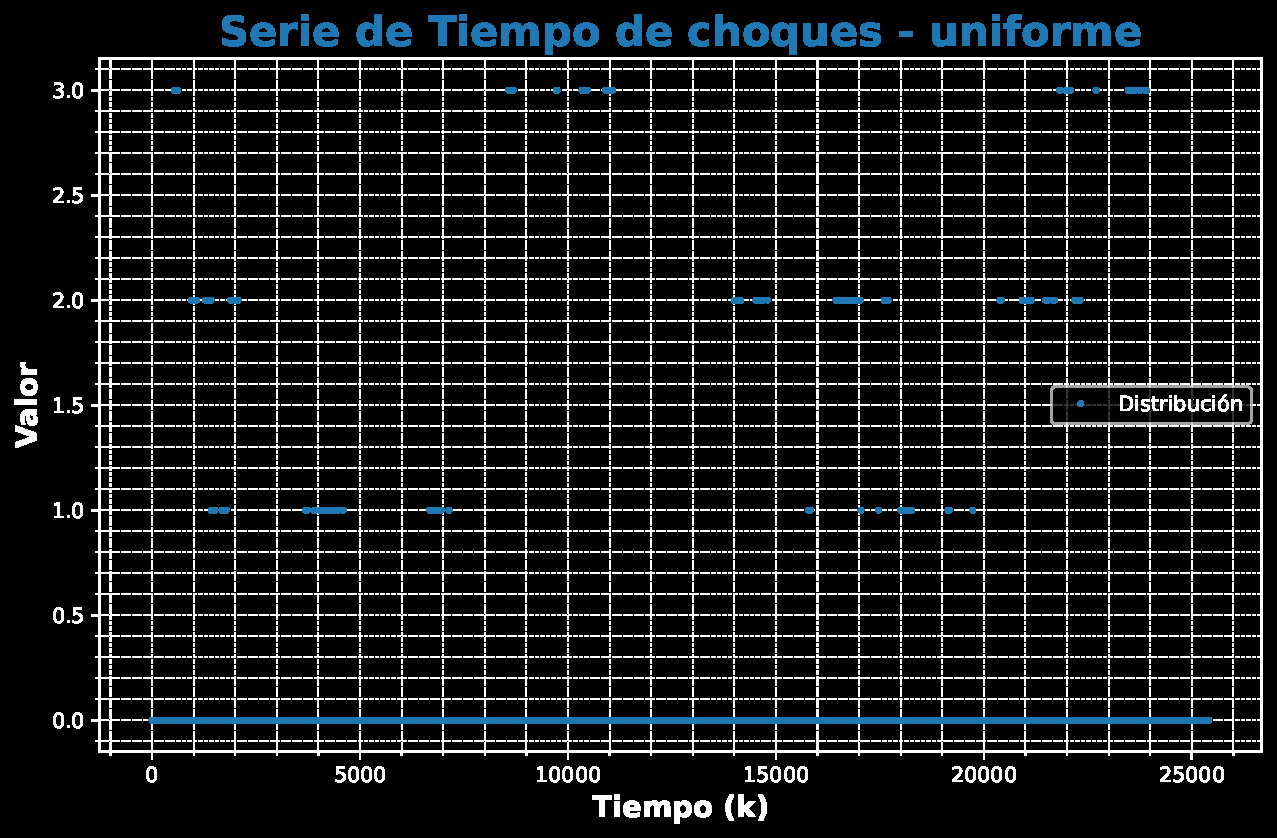
\includegraphics[width=0.7\textwidth]{graf_choques_uniforme.pdf}
	 	\caption{Gráfica de la serie de tiempo para los choques del caminante con distribución normal.}
	 	\label{fig:chUnifGraf}
	 \end{figure}
	 \begin{multicols}{2}
	 	\begin{minipage}{\linewidth}
	 		\centering
	 		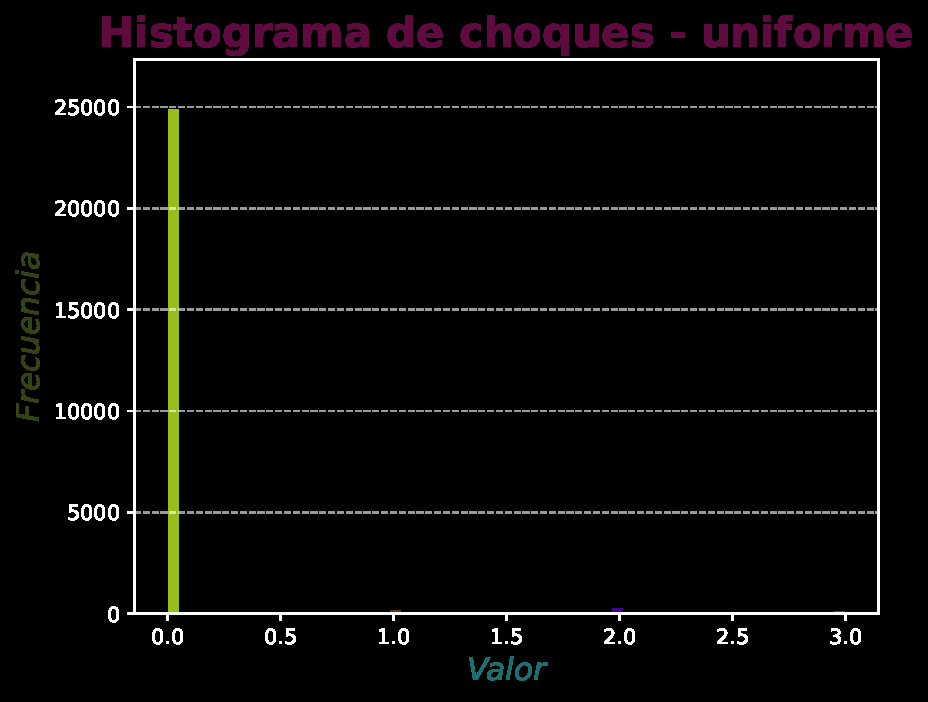
\includegraphics[width=1\linewidth]{hist_choques_uniforme.pdf}
	 		\captionof{figure}{Histograma.}
	 		\label{fig:chUnifHist}
	 	\end{minipage}
	 	\vfill\columnbreak
	 	\begin{minipage}{\linewidth}
	 		\centering
	 		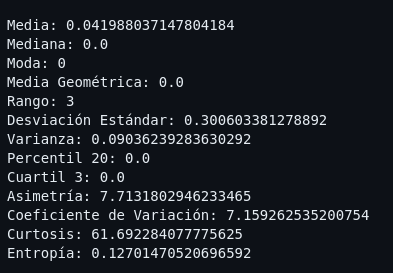
\includegraphics[width=1\linewidth]{u4.png}%
	 		\captionof{figure}{Métricas}
	 		\label{chUnifMet}
	 	\end{minipage}
	 \end{multicols}
	 
	 \begin{itemize}
	 	\item La \textbf{mediana} y la \textbf{moda} de 0 sugieren que la mayor parte de los valores en la serie de tiempo son ceros, lo que puede indicar ausencia de choques durante la mayoría de las observaciones.
	 	\item La \textbf{media geométrica} es 0, lo que confirma que los valores son predominantemente ceros o valores cercanos a cero.
	 	\item La \textbf{desviación estándar} de 0.3006 es relativamente pequeña, lo que indica que hay poca variación en los valores y que la mayoría de los valores están cerca de la media.
	 	\item El \textbf{percentil 20} de 0 refuerza el hallazgo de que al menos el 20\% de los datos son ceros.
	 	\item El \textbf{cuartil 3} de 0 sugiere que hasta el 75\% de los datos podrían ser ceros, lo que refleja la alta frecuencia de valores sin choques en la serie de tiempo.
	 	\item Una \textbf{asimetría} de aproximadamente 7.71 indica una distribución muy sesgada, con una cola hacia valores mayores que la mayoría de las observaciones.
	 	\item El \textbf{coeficiente de variación} de aproximadamente 7.15, al ser relativamente alto, sugiere que la variabilidad de los datos es significativa en comparación con la media, lo cual es notable dado que la media es muy baja.
	 	\item La \textbf{curtosis} extremadamente alta de aproximadamente 61.69 sugiere una distribución con un pico muy pronunciado en cero y colas muy gruesas, lo que indica una concentración significativa de ceros y la presencia de valores atípicos ocasionales.
	 	\item La \textbf{entropía} de 0.1270 es baja, lo que implica una alta predecibilidad en la serie de tiempo, probablemente debido a la gran cantidad de ceros.
	 \end{itemize}
	 
	 Dado el predominio de ceros y la baja variabilidad general con la excepción de algunos valores atípicos, la serie de tiempo presenta características de una distribución donde la mayoría de los eventos no registran un cambio, pero ocasionalmente se observan picos significativos.
	 
	 
	 \newpage
	 \subsection{Caminante Aleatorio con Distribución Normal}
	 \begin{center}
	 	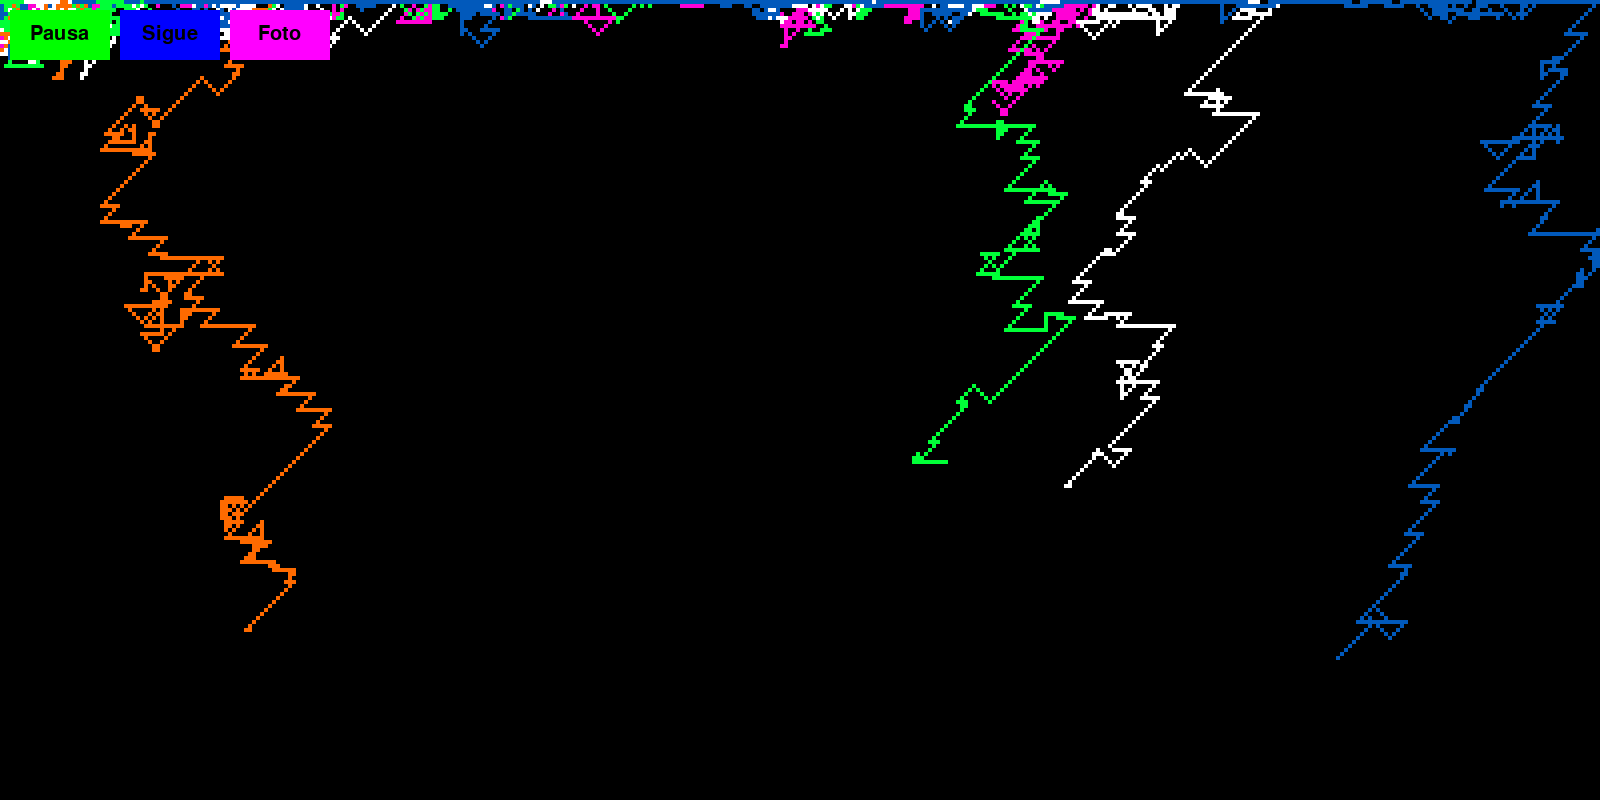
\includegraphics[width=0.65\linewidth]{walkerNormal.png}
	 	\captionof{figure}{Caminante Aleatorio - Distribución Normal}
	 	\label{walkerNormal}
	 \end{center}
	 
 
 	\subsection{Direcciones}
	 \begin{figure}[h]
	 	\centering
	 	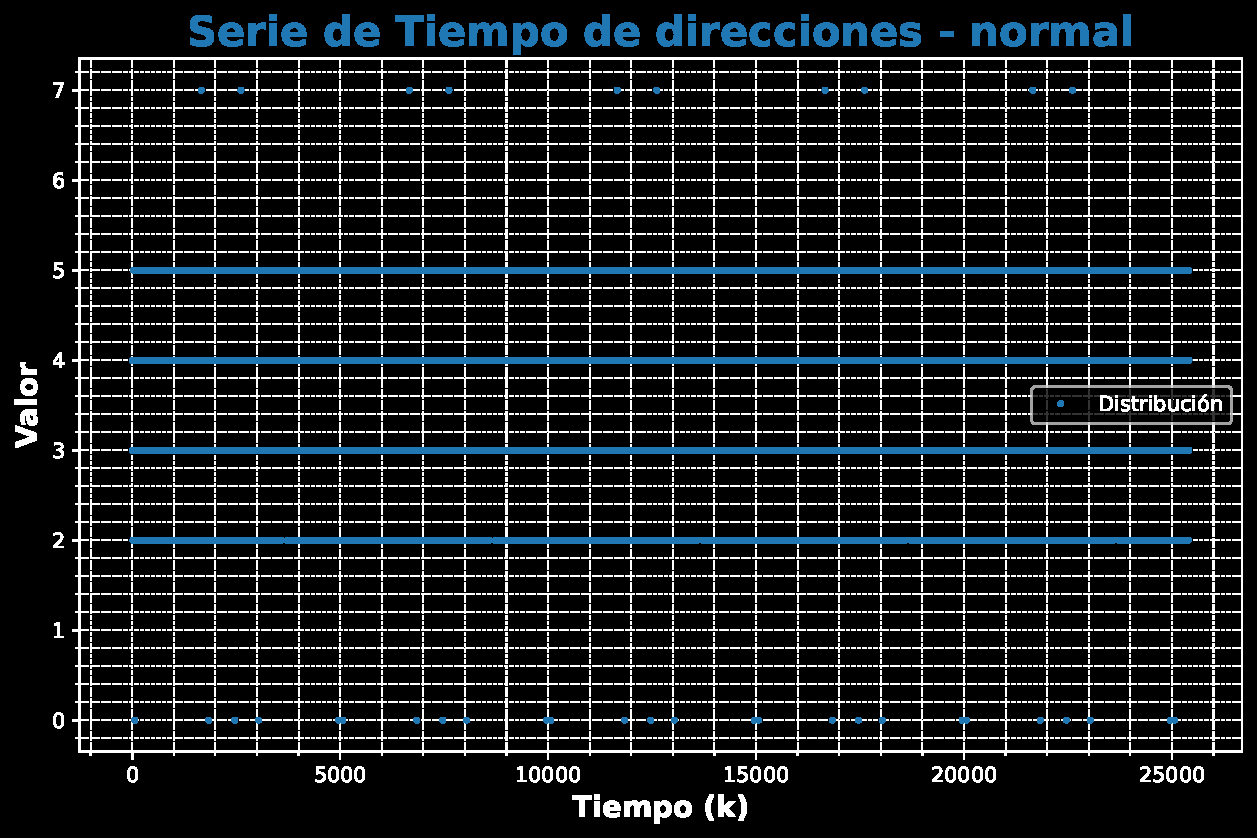
\includegraphics[width=0.6\textwidth]{graf_direcciones_normal.pdf}
	 	\caption{Gráfica de la serie de tiempo para las direcciones del caminante con distribución normal.}
	 	\label{fig:direcNormalGraf}
	 \end{figure}
	 \begin{multicols}{2}
	 	\begin{minipage}{\linewidth}
	 		\centering
	 		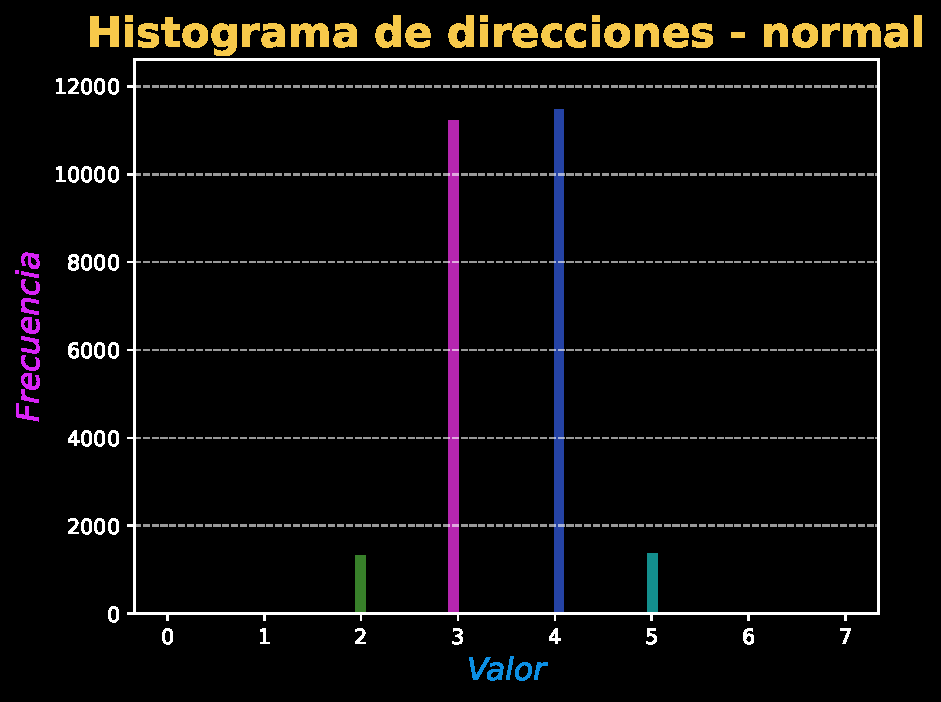
\includegraphics[width=0.9\linewidth]{hist_direcciones_normal.pdf}
	 		\captionof{figure}{Histograma.}
	 		\label{fig:direcNormalHist}
	 	\end{minipage}
	 	\vfill\columnbreak
	 	\begin{minipage}{\linewidth}
	 		\centering
	 		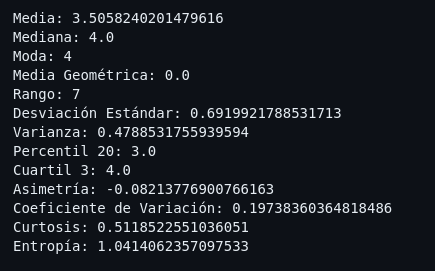
\includegraphics[width=1\linewidth]{n1.png}%
	 		\captionof{figure}{Métricas}
	 		\label{direcNormalMet}
	 	\end{minipage}
	 \end{multicols}
	 
	 \begin{itemize}
	 	\item La \textbf{media} de aproximadamente 3.51 sugiere que el promedio de los valores observados se inclina ligeramente hacia el extremo inferior del rango.
	 	\item La \textbf{mediana} de 4.0 indica que la mitad de los valores son menores que 4 y la otra mitad mayores, apuntando a una distribución equilibrada alrededor de este punto.
	 	\item La \textbf{moda} de 4 señala que el valor más frecuente en la serie de tiempo es 4, lo cual puede indicar una concentración de medidas alrededor de este valor.
	 	\item El \textbf{rango} de 7 muestra la extensión completa desde el valor más bajo al más alto.
	 	\item La \textbf{desviación estándar} de aproximadamente 0.6199 refleja que hay poca dispersión de los valores respecto a la media.
	 	\item La \textbf{varianza} de 0.4788 es una medida de la dispersión que confirma la baja variabilidad de los datos alrededor de la media.
	 	\item La \textbf{asimetría} cercana a cero implica que la serie de tiempo tiene una distribución simétrica.
	 	\item El \textbf{coeficiente de variación} de aproximadamente 0.19 indica una baja variabilidad relativa en relación con la media de la serie de tiempo.
	 	\item Una \textbf{curtosis} negativa de -0.081 sugiere que la serie de tiempo tiene una distribución menos concentrada que la normal, con colas más ligeras.
	 	\item La \textbf{entropía} muy baja de 0.141 implica que hay poca incertidumbre o aleatoriedad en la serie de tiempo, posiblemente debido a una alta frecuencia de valores repetidos o un rango limitado de valores únicos. Además es similar a la típica de la distribución normal: \(\frac{1}{2} \ln(2 \pi e \sigma^2)\) = \(\frac{1}{2} \ln(2 \pi e (0.4788))\) = 1.050
	 \end{itemize}
	 
	 Las métricas indican una serie de tiempo con valores que están normalmente distribuidos o concentrados en torno a un número limitado de estados, dada la baja dispersión y alta frecuencia de ciertos valores.
	 
	 \subsection{Distancias}
	 \begin{figure}[h]
	 	\centering
	 	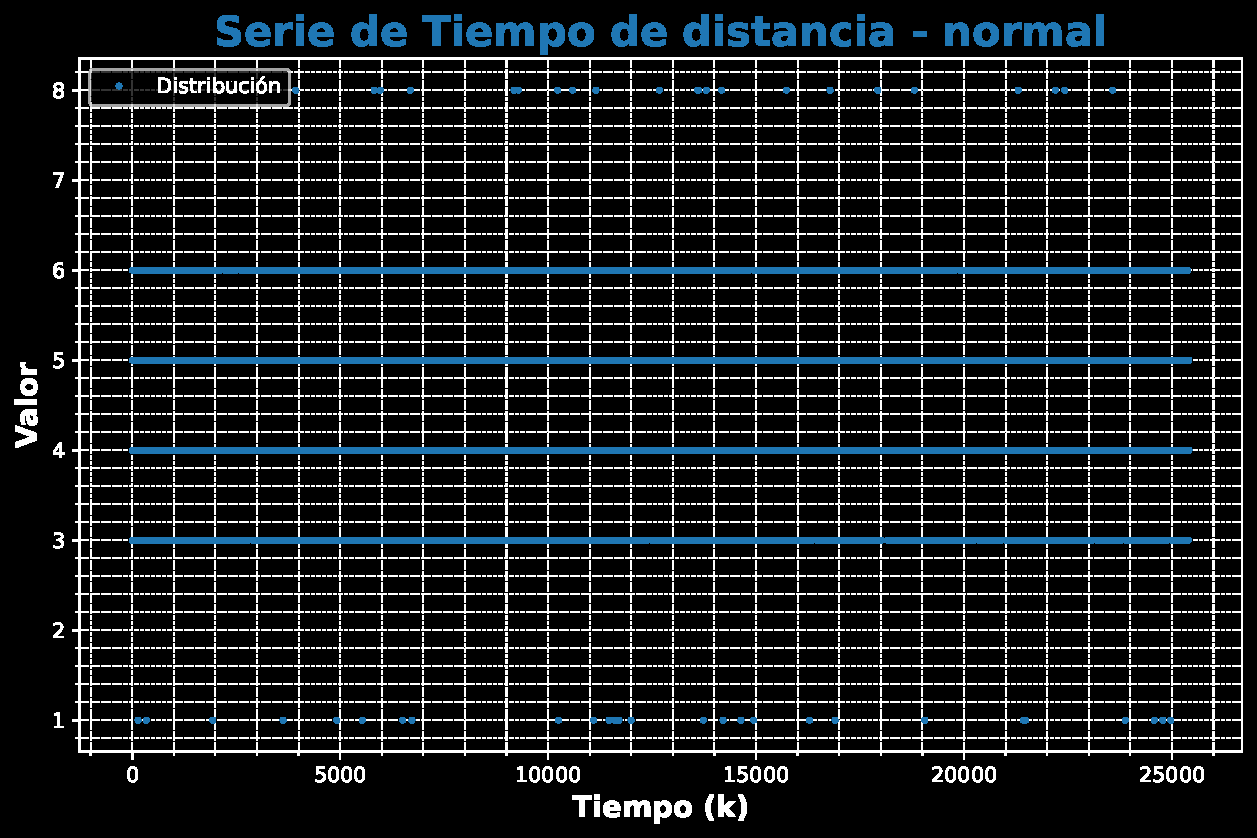
\includegraphics[width=0.6\textwidth]{graf_distancia_normal.pdf}
	 	\caption{Gráfica de la serie de tiempo para las distancias del caminante con distribución normal.}
	 	\label{fig:distNormalGraf}
	 \end{figure}
	 \begin{multicols}{2}
	 	\begin{minipage}{\linewidth}
	 		\centering
	 		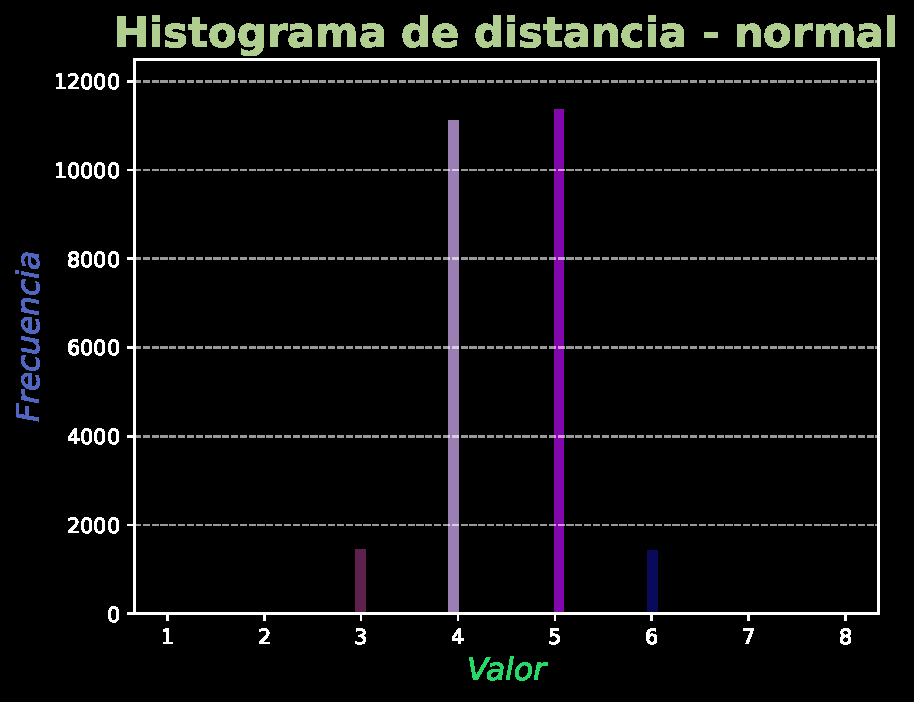
\includegraphics[width=0.9\linewidth]{hist_distancia_normal.pdf}
	 		\captionof{figure}{Histograma.}
	 		\label{fig:distNormalHist}
	 	\end{minipage}
	 	\vfill\columnbreak
	 	\begin{minipage}{\linewidth}
	 		\centering
	 		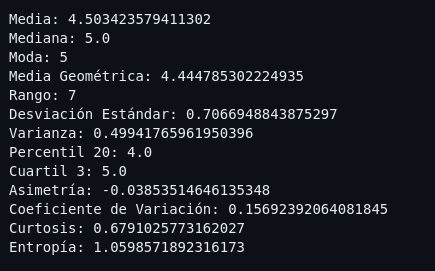
\includegraphics[width=1\linewidth]{n2.png}%
	 		\captionof{figure}{Métricas}
	 		\label{distNormalMet}
	 	\end{minipage}
	 \end{multicols}
	 
	 \begin{itemize}
	 	\item La \textbf{media} de aproximadamente 4.50 sugiere que en promedio, los valores de la serie de tiempo se centran en la mitad del rango de valores posibles.
	 	\item La \textbf{mediana} de 5.0, igual a la moda, indica que la mitad de las mediciones son menores que 5 y la otra mitad mayores, apoyando la presencia de una distribución equilibrada alrededor de este valor central.
	 	\item La \textbf{moda} de 5, coincidiendo con la mediana y la media, apunta a que es el valor más frecuente, lo que podría indicar un pico en la distribución de los datos.
	 	\item La \textbf{media geométrica} de aproximadamente 4.44 está cerca de la media, lo que sugiere que los valores bajos no dominan la serie de tiempo.
	 	\item El \textbf{rango} de 7 indica la extensión total desde el valor más bajo al más alto en la serie de tiempo.
	 	\item La \textbf{desviación estándar} de aproximadamente 0.77 muestra que los valores tienden a variar moderadamente alrededor de la media.
	 	\item La \textbf{varianza} de cerca de 0.49 como el cuadrado de la desviación estándar, refleja esta dispersión de los valores.
	 	\item La \textbf{asimetría} cercana a cero sugiere que la serie de tiempo es simétrica.
	 	\item El \textbf{coeficiente de variación} de aproximadamente 0.17 indica una baja variabilidad relativa respecto a la media.
	 	\item La \textbf{entropía} de aproximadamente 1.06, algo baja, sugiere que hay un grado de predecibilidad en la serie de tiempo.  Además es similar a la típica de la distribución normal: \(\frac{1}{2} \ln(2 \pi e \sigma^2)\) = \(\frac{1}{2} \ln(2 \pi e (0.4994))\) = 1.071
	 \end{itemize}
	 
	 Dado el pico pronunciado en la moda y la simetría reflejada en las métricas, junto con la baja entropía y una ligera puntiagudez indicada por la curtosis, las métricas sugieren que la serie de tiempo podría estar distribuida de manera normal con una tendencia a agruparse alrededor de un punto central. Esto es consistente con el histograma que muestra un pico en el valor central con una distribución simétrica a su alrededor.
	 
	 
	 \subsection{Posiciones}
	 \begin{figure}[h]
	 	\centering
	 	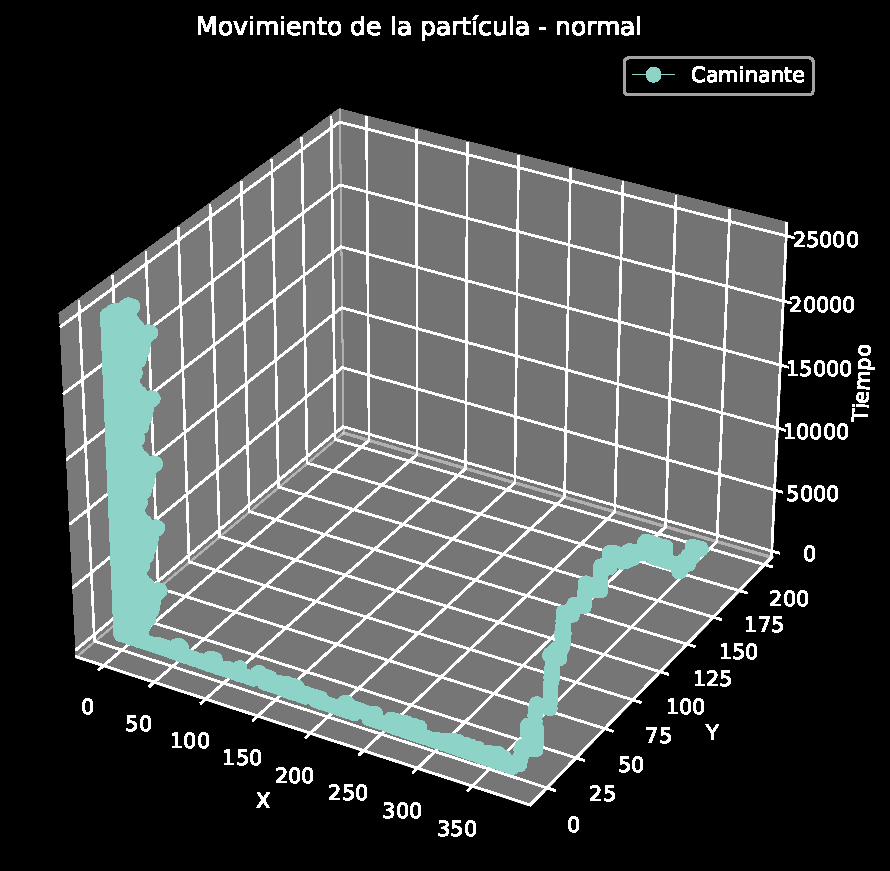
\includegraphics[width=0.45\textwidth]{graf_posiciones_normal.pdf}
	 	\caption{Gráfica de la serie de tiempo para las posiciones del caminante con distribución normal.}
	 	\label{fig:posNormalGraf}
	 \end{figure}
	 \begin{multicols}{2}
	 	\begin{minipage}{\linewidth}
	 		\centering
	 		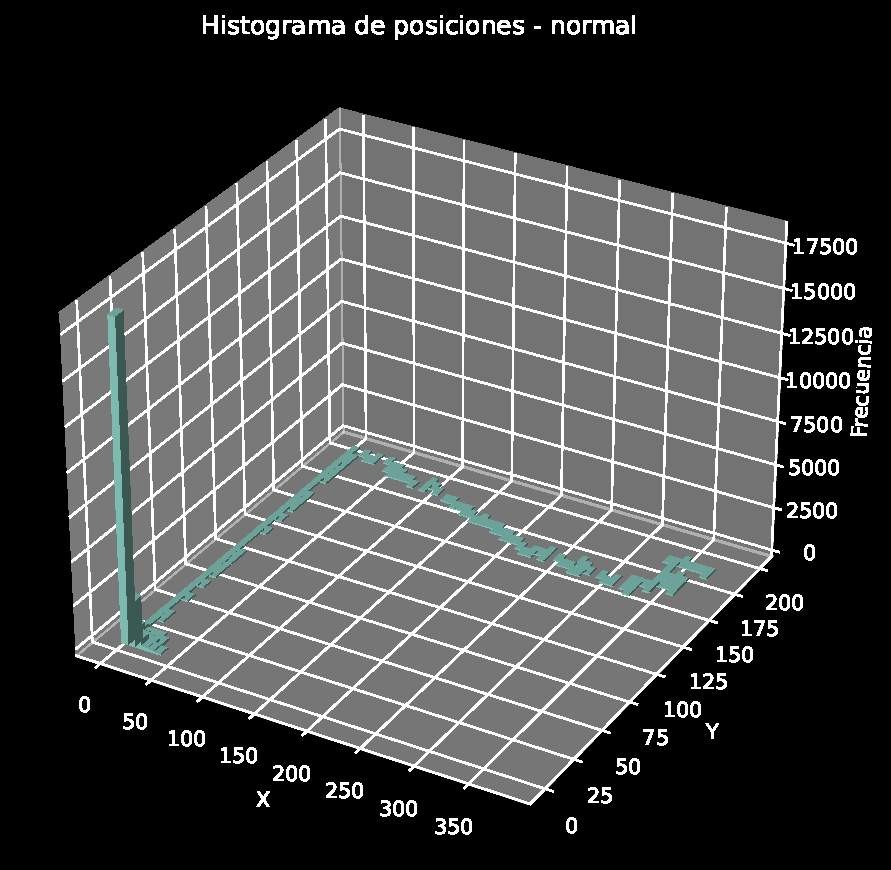
\includegraphics[width=0.8\linewidth]{hist_posiciones_normal.pdf}
	 		\captionof{figure}{Histograma.}
	 		\label{fig:posNormalHist}
	 	\end{minipage}
	 	\vfill\columnbreak
	 	\begin{minipage}{\linewidth}
	 		\centering
	 		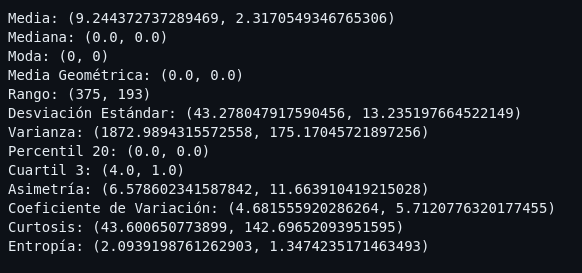
\includegraphics[width=1\linewidth]{n3.png}%
	 		\captionof{figure}{Métricas}
	 		\label{posNormalMet}
	 	\end{minipage}
	 \end{multicols}
	 \begin{itemize}
	 	\item La \textbf{media} con coordenadas (9.24, 2.32) sugiere un centro de masa para las posiciones que tiende a estar en la parte inferior izquierda del rango de los datos.
	 	\item Las \textbf{medianas} y \textbf{modas} de (0, 0) indican que el valor más común y el valor medio de las posiciones están en el origen, lo cual podría sugerir una concentración de posiciones o un punto de partida común.
	 	\item La \textbf{media geométrica} también de (0, 0) confirma la influencia de valores bajos en los datos, posiblemente debido a la frecuencia de ceros en las posiciones.
	 	\item El \textbf{rango} en las coordenadas (375, 193) muestra la extensión total de los datos a lo largo de las direcciones x e y.
	 	\item La \textbf{desviación estándar} con valores (14.23, 13.23) refleja una dispersión considerable de las posiciones alrededor del centro de masa.
	 	\item La \textbf{asimetría} con valores (6.57, 4.65) indica una distribución con colas pesadas que se extienden hacia valores mayores en ambas direcciones x e y.
	 	\item El \textbf{coeficiente de variación} con valores (1.54, 5.70) sugiere una alta variabilidad relativa, especialmente en la dirección y.
	 	\item La \textbf{curtosis} extremadamente alta en las coordenadas (43.69, 642.65) implica una distribución con picos muy pronunciados y colas muy gruesas en ambas direcciones.
	 \end{itemize}
	 
	 Dadas las métricas, la serie de tiempo podría reflejar un comportamiento donde las posiciones están altamente concentradas cerca del origen, con ocasionales valores atípicos que generan una distribución con colas largas y picos pronunciados. Esto puede ser indicativo de un proceso con un estado o ubicación de inicio común, seguido de movimientos que, aunque infrecuentes, pueden ser de gran magnitud.
	
	
	\subsection{Choques con pared}
	 \begin{figure}[h]
	 	\centering
	 	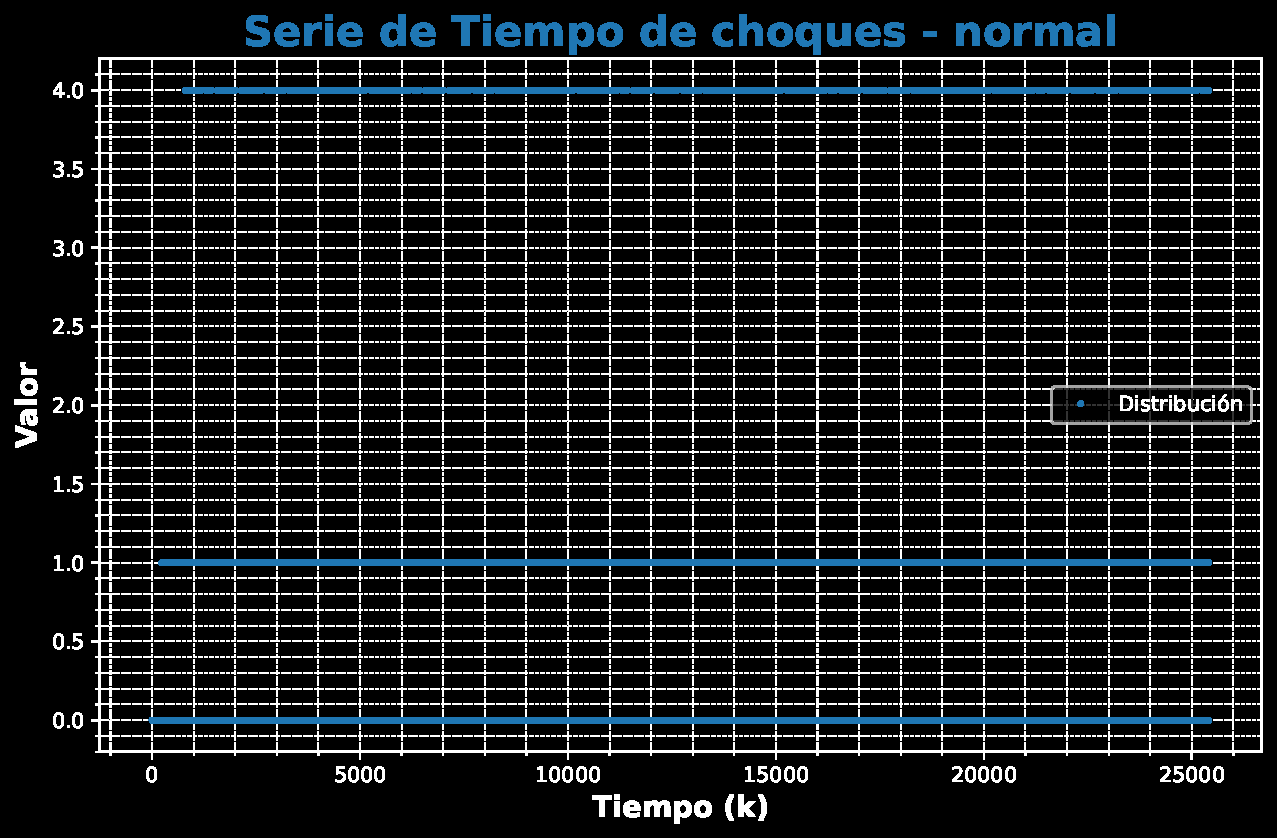
\includegraphics[width=0.5\textwidth]{graf_choques_normal.pdf}
	 	\caption{Gráfica de la serie de tiempo para las choques del caminante con distribución normal.}
	 	\label{fig:chNormalGraf}
	 \end{figure}
	 \begin{multicols}{2}
	 	\begin{minipage}{\linewidth}
	 		\centering
	 		\includegraphics[width=0.9\linewidth]{hist_choques_normal.pdf}
	 		\captionof{figure}{Histograma.}
	 		\label{fig:chNormalHist}
	 	\end{minipage}
	 	\vfill\columnbreak
	 	\begin{minipage}{\linewidth}
	 		\centering
	 		\includegraphics[width=1\linewidth]{n4.png}%
	 		\captionof{figure}{Métricas}
	 		\label{chNormalMet}
	 	\end{minipage}
	 \end{multicols}
	 
	 \begin{itemize}
	 	\item La \textbf{media} de aproximadamente 0.809 indica que, en promedio, los choques ocurren en la pared 1.
	 	\item La \textbf{mediana} y la \textbf{moda} de 1.0 sugieren que la mayoría de las observaciones de la serie de tiempo registran un solo choque.
	 	\item La \textbf{media geométrica} de 0.0 refuerza la presencia de valores cero en los datos, lo que indica periodos sin choques.
	 	\item La \textbf{desviación estándar} de aproximadamente 0.974 muestra una variabilidad moderada de la frecuencia de los choques alrededor de la media.
	 	\item El \textbf{percentil 20} de 0.0 implica que al menos el 20\% de los choques registrados son cero, lo que sugiere que no hay choques durante ese porcentaje de tiempo.
	 	\item El \textbf{cuartil 3} de 1.0 indica que el 75\% de los choques tienen presencia en la pared 1.
	 	\item La \textbf{asimetría} de aproximadamente 2.10 sugiere una distribución sesgada hacia valores más bajos, con colas más pesadas hacia valores mayores.
	 	\item El \textbf{coeficiente de variación} de aproximadamente 1.20 indica una alta variabilidad relativa en relación con la media.
	 	\item Una \textbf{curtosis} de aproximadamente 4.81 indica una distribución con un pico pronunciado y colas pesadas.
	 	\item La \textbf{entropía} de 0.877, más baja que 1, sugiere una distribución con cierta predecibilidad y la presencia de un valor común o repetitivo.
	 \end{itemize}
	 
	 La combinación de la moda y mediana en 1, junto con la alta asimetría y curtosis, y una media relativamente baja, sugiere que los choques ocurren mayor frecuencia en la pared 1, aunque puede no haberlos esporádicamente.
	
	
	
	\newpage	
	\subsection{Caminante Aleatorio con Distribución Gamma}
	\begin{center}
		\includegraphics[width=0.7\linewidth]{walkerGamma.png}
		\captionof{figure}{Caminante Aleatorio - Distribución Gamma}
		\label{walkerGamma}
	\end{center}
	
	\subsection{Direcciones}
	\begin{figure}[h]
		\centering
		\includegraphics[width=0.55\textwidth]{graf_direcciones_gamma.pdf}
		\caption{Gráfica de la serie de tiempo para las direcciones del caminante con distribución gamma.}
		\label{fig:direcGammaGraf}
	\end{figure}
	\begin{multicols}{2}
		\begin{minipage}{\linewidth}
			\centering
			\includegraphics[width=1\linewidth]{hist_direcciones_gamma.pdf}
			\captionof{figure}{Histograma.}
			\label{fig:direcGammaHist}
		\end{minipage}
		\vfill\columnbreak
		\begin{minipage}{\linewidth}
			\centering
			\includegraphics[width=1\linewidth]{g1.png}%
			\captionof{figure}{Métricas}
			\label{direcGammaMet}
		\end{minipage}
	\end{multicols}
	
	\begin{itemize}
		\item La \textbf{media} cercana a 0.41 sugiere que la mayoría de los valores en la serie de tiempo tienen una tendencia hacia la dirección 0.
		\item Tanto la \textbf{mediana} como la \textbf{moda} son 0, indicando que el valor más frecuente y el punto medio de los datos es cero, lo que sugiere una alta frecuencia de eventos en esta dirección.
		\item La \textbf{media geométrica} es 0, lo cual es coherente con una alta proporción de valores cero en la serie de tiempo.
		\item El \textbf{rango} de 7 indica que, aunque el caminante se mueve más hacia la dirección 0, ocasionalmente también lo hace en las direcciones 1 a 7.
		\item La \textbf{desviación estándar} de aproximadamente 0.7268 señala una variabilidad moderada de los datos desde la media.
		\item El \textbf{percentil 20} es 0, lo que refuerza la presencia de muchos valores que apuntan a la dirección 0 en la serie de tiempo.
		\item El \textbf{cuartil 3} de 1 muestra que hasta el 75\% de los datos tienen valores en las direcciones 0 o 1.
		\item La \textbf{asimetría} positiva de aproximadamente 2.33 indica una distribución con una cola más larga hacia los valores mayores.
		\item El \textbf{coeficiente de variación} de aproximadamente 1.76 muestra una variabilidad relativa alta en comparación con la media, que es un indicador de que los valores más altos son menos frecuentes pero significativamente diferentes de la mayoría de los valores.
		\item Una \textbf{curtosis} alta de aproximadamente 8.07 indica una distribución con colas más pesadas y un pico más pronunciado alrededor del cero.
		\item La \textbf{entropía} de aproximadamente 0.84, aunque más alta que en una distribución con una sola moda, sigue siendo relativamente baja, lo que indica un cierto grado de regularidad en la serie de tiempo.
	\end{itemize}
	
	La combinación de una media baja, una alta frecuencia de ceros y una asimetría positiva con una curtosis alta sugiere que la serie de tiempo puede caracterizarse por una distribución gamma, con gran cantidad de eventos en la dirección cero. Esto podría reflejar un proceso donde el movimiento o el cambio es generalmente mínimo, con algunos picos esporádicos de actividad más alta.
	
	
	
	\newpage
	\subsection{Distancias}
	\begin{figure}[h]
		\centering
		\includegraphics[width=0.6\textwidth]{graf_distancia_gamma.pdf}
		\caption{Gráfica de la serie de tiempo para las distancias del caminante con distribución gamma.}
		\label{fig:distGammaGraf}
	\end{figure}
	\begin{multicols}{2}
		\begin{minipage}{\linewidth}
			\centering
			\includegraphics[width=1\linewidth]{hist_distancia_gamma.pdf}
			\captionof{figure}{Histograma.}
			\label{fig:distGammaHist}
		\end{minipage}
		\vfill\columnbreak
		\begin{minipage}{\linewidth}
			\centering
			\includegraphics[width=1\linewidth]{g2.png}%
			\captionof{figure}{Métricas}
			\label{distGammaMet}
		\end{minipage}
	\end{multicols}
	
	\begin{itemize}
		\item La \textbf{media} de 1.41 sugiere que el valor promedio de las distancias es moderado dentro del rango de datos.
		\item Tanto la \textbf{mediana} como la \textbf{moda} son 1, lo que indica una concentración de valores alrededor de este punto. Esto puede significar que la mayoría de las distancias son consistentemente bajas, con menos instancias de distancias más largas.
		\item La \textbf{media geométrica} de aproximadamente 1.28 es consistente con la presencia de valores no nulos, indicando que la distribución no está sesgada hacia el cero.
		\item El \textbf{rango} de 7 muestra la diferencia entre las distancias más cortas y más largas observadas.
		\item Una \textbf{desviación estándar} de aproximadamente 0.74 sugiere que hay una variación moderada de las distancias alrededor de la media.
		\item El \textbf{percentil 20} de 1 indica que al menos el 20\% de los valores son 1 o menos.
		\item El \textbf{cuartil 3} de 2 muestra que el 75\% de las distancias son 2 o menos, lo que apoya la existencia de una concentración de valores bajos.
		\item Una \textbf{asimetría} de aproximadamente 2.29 sugiere una cola más pesada hacia las distancias más largas.
		\item El \textbf{coeficiente de variación} de 0.52 indica que la variabilidad de las distancias es más de la mitad de la media, lo cual es notablemente alta.
		\item Una \textbf{curtosis} de aproximadamente 7.17 indica que la distribución es cuenta con un pico más pronunciado que una distribución normal y colas más pesadas.
		\item La \textbf{entropía} de 0.85 es relativamente baja, lo que podría sugerir cierta regularidad o predictibilidad en las distancias observadas.
	\end{itemize}
	
	Estas métricas pueden indicar que, mientras que la mayoría de las distancias en la serie de tiempo son bajas, hay una cantidad significativa de instancias con distancias más altas. La presencia de una asimetría positiva y una curtosis alta sugiere que esas distancias más altas, aunque raras, pueden ser extremadamente altas en comparación con la mayoría de los datos. La baja entropía y la media geométrica mayor que cero sugieren que hay una tendencia general hacia distancias más bajas, pero con eventos intermitentes de distancias más largas, como se encontraría en una distribución gamma.
	
	
	\subsection{Posiciones}
	\begin{figure}[h]
		\centering
		\includegraphics[width=0.5\textwidth]{graf_posiciones_gamma.pdf}
		\caption{Gráfica de la serie de tiempo para las posiciones del caminante con distribución gamma.}
		\label{fig:posGammaGraf}
	\end{figure}
	\begin{multicols}{2}
		\begin{minipage}{\linewidth}
			\centering
			\includegraphics[width=0.8\linewidth]{hist_posiciones_gamma.pdf}
			\captionof{figure}{Histograma.}
			\label{fig:posGammaHist}
		\end{minipage}
		\vfill\columnbreak
		\begin{minipage}{\linewidth}
			\centering
			\includegraphics[width=1\linewidth]{g3.png}%
			\captionof{figure}{Métricas}
			\label{posGammaMet}
		\end{minipage}
	\end{multicols}
	
	\begin{itemize}
		\item La \textbf{media} en las coordenadas (392.09, 0.25) indica que, en promedio, las posiciones registradas tienden a ser cercanas a estas coordenadas, con una concentración significativa en la dirección 'x'.
		\item La \textbf{mediana} y la \textbf{moda} en las coordenadas (399, 0) muestran que la mayoría de las observaciones se acumulan en este punto específico del espacio, lo que podría indicar un lugar de alta frecuencia o un punto de estancia común.
		\item La \textbf{media geométrica} en (389.36, 0) sugiere que los valores de la serie de tiempo tienen una tendencia multiplicativa hacia estas coordenadas, excluyendo los valores de cero.
		\item El \textbf{rango} de (293, 73) muestra la extensión total en el espacio de las coordenadas 'x' e 'y'.
		\item La \textbf{desviación estándar} en (35.65, 2.96) indica una dispersión considerable alrededor de la media en ambas direcciones, especialmente en 'x'.
		\item La \textbf{varianza} en (1271.54, 8.79) cuantifica esta dispersión y confirma la variabilidad significativa en 'x' y una menor en 'y'.
		\item El \textbf{cuartil 3} en (399, 0) sugiere que hasta el 75\% de las observaciones caen dentro o por debajo de estas coordenadas.
		\item La \textbf{asimetría} en (3.53, 9.17) indica una distribución sesgada, con una cola más larga hacia los valores mayores en ambas coordenadas.
		\item La \textbf{curtosis} extremadamente alta en (35.42, 903.18) implica una distribución con picos muy pronunciados cerca de las modas y colas gruesas, indicando una alta frecuencia de valores comunes y la presencia de valores atípicos significativos.
		\item La \textbf{entropía} baja en (0.66, 0.34) sugiere un cierto grado de regularidad o predecibilidad en la distribución de las posiciones, especialmente en 'y'.
	\end{itemize}
	
	La alta concentración de valores en la coordenada 'x' cerca de 399 y la moda y mediana en cero para 'y', junto con la gran curtosis, indican que la serie de tiempo presenta una distribución donde hay un comportamiento dominante o un estado estacionario que el caminante ocupa con frecuencia, con variaciones ocasionales que pueden ser extremas. La baja entropía en la coordenada 'y' puede reflejar que el caminante cambia de posición en 'y' con menos frecuencia o dentro de un rango más limitado de valores.
	
	
	\subsection{Choques con pared}
	\begin{figure}[h]
		\centering
		\includegraphics[width=0.6\textwidth]{graf_choques_gamma.pdf}
		\caption{Gráfica de la serie de tiempo para los choques del caminante con distribución gamma.}
		\label{fig:chGammaGraf}
	\end{figure}
	\begin{multicols}{2}
		\begin{minipage}{\linewidth}
			\centering
			\includegraphics[width=1\linewidth]{hist_choques_gamma.pdf}
			\captionof{figure}{Histograma.}
			\label{fig:chGammaHist}
		\end{minipage}
		\vfill\columnbreak
		\begin{minipage}{\linewidth}
			\centering
			\includegraphics[width=1\linewidth]{g4.png}%
			\captionof{figure}{Métricas}
			\label{chGammaMet}
		\end{minipage}
	\end{multicols}


\begin{itemize}
	\item La \textbf{media} de aproximadamente 0.85 sugiere que, en promedio, el número de choques se encuentra en la pared 1.
	\item La \textbf{mediana} y la \textbf{moda} iguales a 1 reflejan que el valor más comúnmente observado y el valor central de la distribución de choques es 1.
	\item El \textbf{rango} de 2 muestra que las paredes de los choques oscilan entre la 1 y 2.
	\item Una \textbf{desviación estándar} baja de 0.39 indica que la mayoría de los choques tienden a estar cerca de la pared 1.
	\item El \textbf{percentil 20} de 1 sugiere que al menos el 20\% de los choques se encuentran en la pared 1.
	\item El \textbf{cuartil 3} también de 1 indica que hasta el 75\% de los choques tienden a estar en esta pared, mostrando una alta concentración de los datos en este valor.
	\item La \textbf{asimetría} negativa de aproximadamente -1.23 sugiere que hay una cola más pesada hacia el extremo inferior de la distribución, es decir, hay más choques en paredes menores que la media (es decir,, sin choques).
	\item Una \textbf{curtosis} de aproximadamente 1.71 sugiere una distribución con un pico más pronunciado que una distribución normal y colas moderadamente pesadas.
\end{itemize}

La combinación de la moda y la mediana en 1, junto con la baja media y la asimetría negativa, sugiere que la serie de tiempo de choques tiene una tendencia a los valores de la pared 1, indicando una concentración de choques alrededor de la pared 1 y baja frecuencia de eventos extremos.

\newpage
\section{Conclusiones}

A lo largo de este proyecto, hemos llevado a cabo un análisis exhaustivo de sistemas dinámicos estocásticos utilizando series de tiempo para caracterizar procesos y determinar su conformidad con distribuciones de probabilidad conocidas. Nuestro enfoque se centró en la generación de datos simulados y en la aplicación de técnicas estadísticas para extraer métricas clave que describen la naturaleza de los procesos subyacentes.

Hemos observado que, mediante la interpretación de la media, la mediana, la moda, la desviación estándar, la varianza, y otras medidas de tendencia central y dispersión, es posible obtener una comprensión detallada de la dinámica de los sistemas. Las métricas de asimetría y curtosis nos permitieron comprender las desviaciones de las distribuciones normales y detectar la presencia de comportamientos atípicos o de colas pesadas en la distribución de eventos.

El uso del coeficiente de variación y de la entropía resultó ser herramientas valiosas en la evaluación de la regularidad y predecibilidad de los procesos. A través del análisis, identificamos patrones recurrentes y movimientos aleatorios que se ajustan a diversas distribuciones de probabilidad, desde uniformes hasta gamma, reflejando la diversidad y la complejidad de los sistemas estudiados.

Este trabajo demuestra la utilidad de las series de tiempo y el análisis estadístico en la descripción cuantitativa de sistemas estocásticos. Las implicaciones de estos hallazgos son amplias, abarcando desde la física teórica hasta las aplicaciones financieras, y proporcionan una base sólida para futuras investigaciones y aplicaciones prácticas en la modelización de sistemas complejos.




\newpage
\section{Anexos}

A continuación se colocan los enlaces a cada uno de los \texttt{notebooks} en donde se programa cada una de las secciones de este proyecto:

\begin{itemize}
	\item \texttt{Generación de números aleatorios con distribución uniforme}:
	
	\href{https://colab.research.google.com/drive/1OqFebhbSkwtjnMdEeamEgZu9fpV-zu0s?usp=sharing}{\textit{https://colab.research.google.com/drive/1OqFebhbSkwtjnMdEeamEgZu9fpV-zu0s?usp=sharing}}.
	
	
	\item \texttt{Tranformación de distribuciones, métricas y sistemas estocásticos}:
	
	\href{https://colab.research.google.com/drive/1bUJ5eagMzJExHf9ogONdEHd8UiY8B5Te?usp=sharing}{\textit{https://colab.research.google.com/drive/1bUJ5eagMzJExHf9ogONdEHd8UiY8B5Te?usp=sharing}}.
	
	
	\item \texttt{Código de la animación del caminante aleatorio}:
	
	\href{https://drive.google.com/file/d/1WpIbDuXZSVaNsdErKyaxrz4aqWC-oSy9/view?usp=sharing}{\textit{https://drive.google.com/file/d/1WpIbDuXZSVaNsdErKyaxrz4aqWC-oSy9/view?usp=sharing}}.
	
	
	\item \texttt{Cálculo de las métricas del caminante aleatorio}:
	
	\href{https://colab.research.google.com/drive/15WKghgRJQMI1qNjLo5keUrGBhxV8Y-Ps?usp=sharing}{\textit{https://colab.research.google.com/drive/15WKghgRJQMI1qNjLo5keUrGBhxV8Y-Ps?usp=sharing}}.
\end{itemize}






\end{document}
